\chapter{Работа №2. Работа с жидкокристаллическим индикатором}
Цель работы: 
\begin{itemize}
\item Изучение принципов работы ЖКИ.
\item Знакомство с регистрами контроллера ЖКИ, регистрами портов микроконтроллера.
\item Разработка программы для микроконтроллера без использования и с использованием SPL.
\end{itemize}

\section{Общие сведения}

На отладочной плате STM32L-Discovery установлен жидкокристаллический индикатор (ЖКИ, англ. LCD. Liquid crystal display), имеющий шесть 14 сегментных знаков, 4 знака двоеточия (Colon), 4 точки (DP), 4 полоски (Bar). Все сегменты объединены в группы СOM0, COM1, COM2, COM3 по 24 сегмента. Каждая группа имеет свой отдельный <<общий провод>>.

\begin{figure}[h!]
\begin{center}
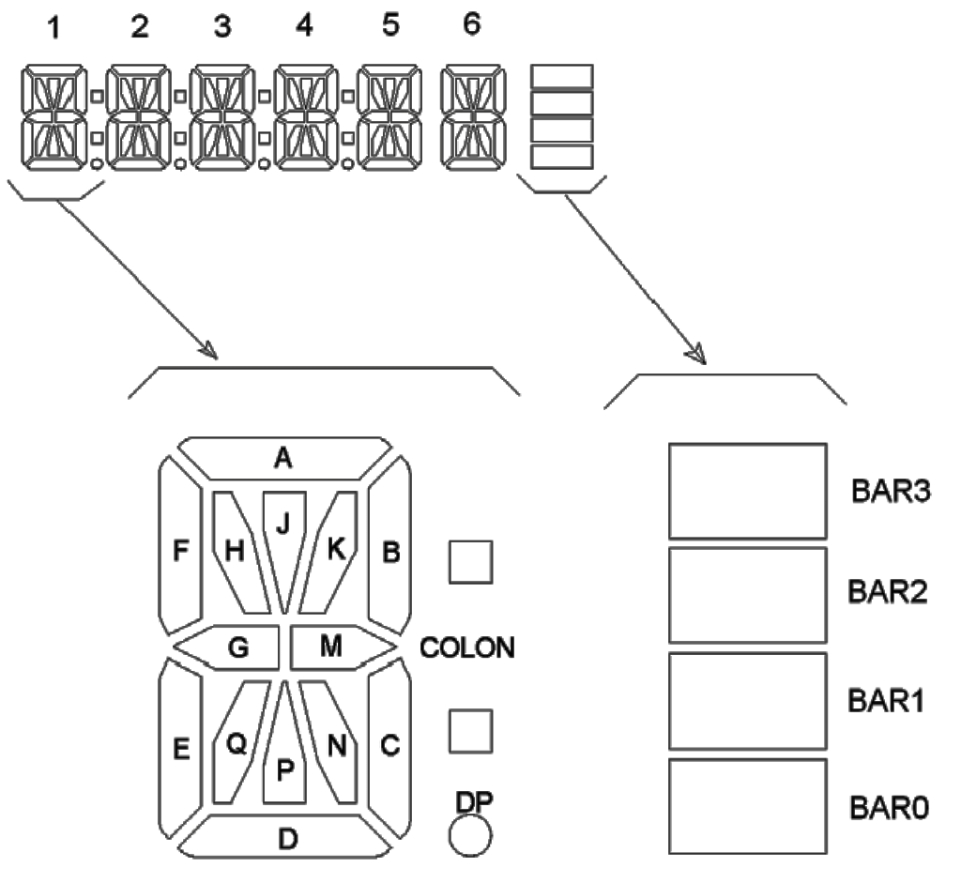
\includegraphics[scale=0.4]{Image/23.jpg}
\end{center}

\caption{Обозначение сегментов ЖКИ}
\end{figure}

\section{Контроллер ЖКИ}
\subsection{Основные функции}
В микроконтроллере есть встроенный контроллер ЖКИ \cite{datasheet}, который управляет монохромными жидкокристаллическими индикаторами. Контроллер ЖКИ:
\begin{enumerate}
\item Позволяет настраивать частоту обновлений (частоту кадров -- частота, с которой обновляется информация на ЖКИ)
\item Поддерживает статический и мультиплексный режим управления.
\item Поддерживает программную установку контраста.
\item Позволяет использовать несколько уровней управляющего напряжения (до четырех)
\item Использует двойную буферизацию, позволяющую обновлять данные в регистрах \textit{LCD\_RAM} в любое время выполнения программы, не нарушая целостность отображаемой информации.
\end{enumerate}

\begin{figure}[h!]
\begin{center}
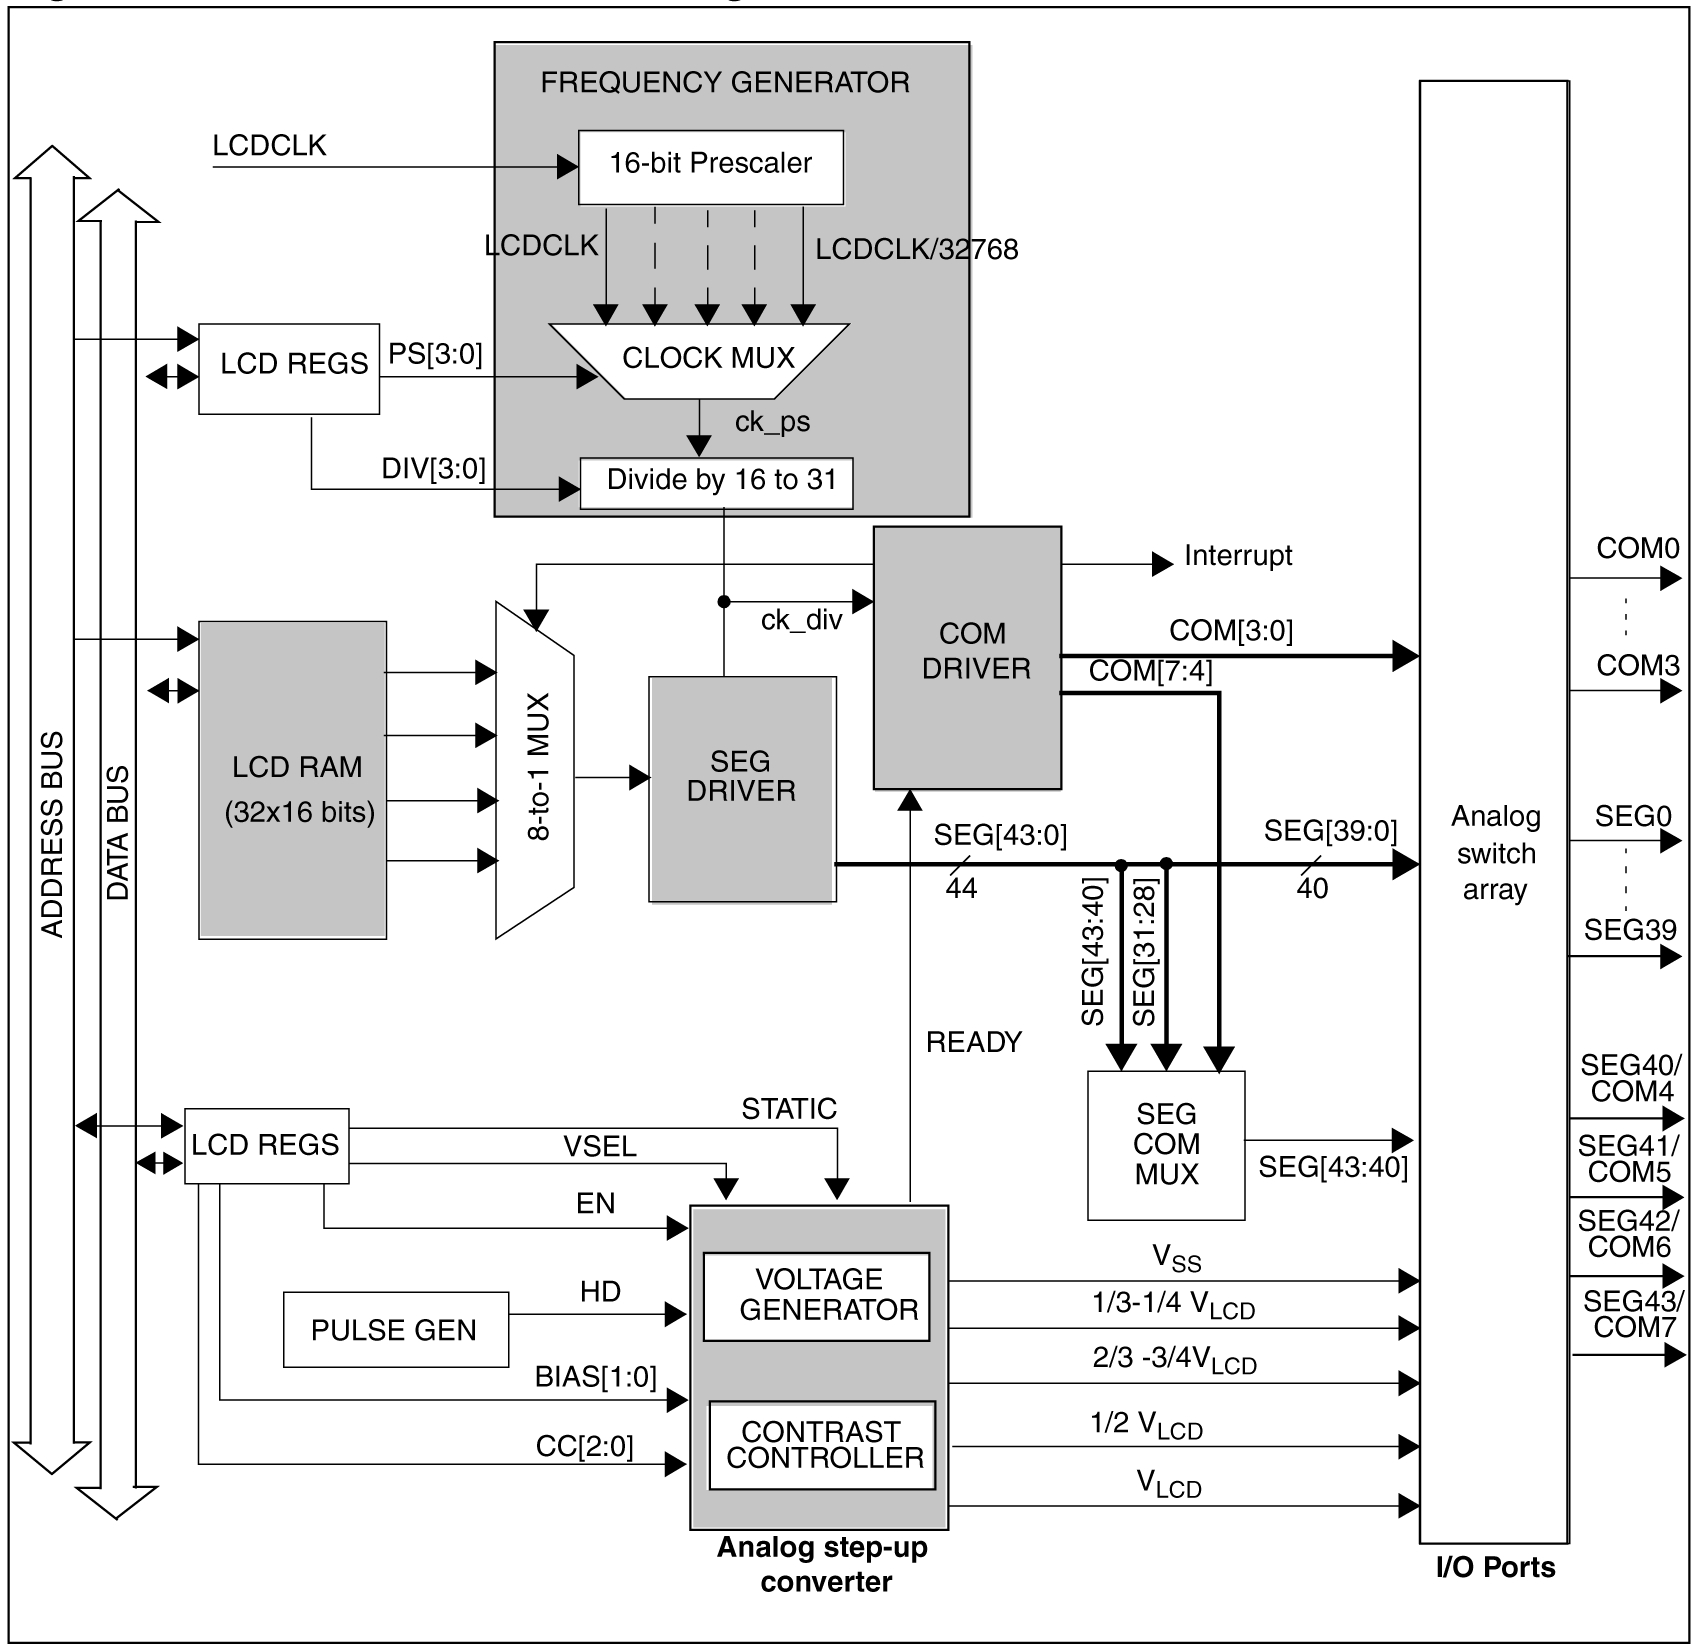
\includegraphics[scale=0.25]{Image/24.jpg}
\end{center}
\caption{Контроллер ЖКИ}
\end{figure}

\subsection{Регистры памяти контроллера ЖКИ}
\label{RegMemLCD}

В микроконтроллере STM32L152RB выделены специальные регистры \textit{LCD\_RAM} \cite{ReferManual}, информация, хранимая в которых, соответствует группе сегментов COM0 -- COM3. Каждой группе соответствует два 32 разрядных регистра. Такое количество регистров позволяет микроконтроллеру управлять ЖКИ c большим количеством сегментов, чем установленным на отладочной плате \cite{chip}.


\begin{figure}[h!]
\begin{center}
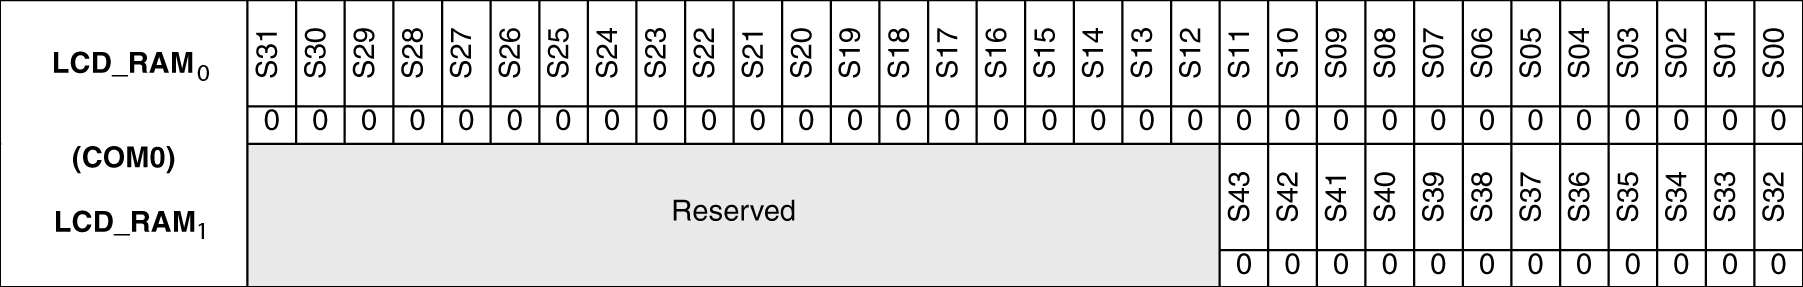
\includegraphics[scale=0.27]{Image/25.jpg}
\end{center}
\caption{Состав группы COM0}\label{COM0}
\end{figure}

Для управления ЖКИ со 176 сегментами используются 4 группы COM0 -- COM3 по 44 сегмента каждая, для управления ЖКИ с 320 сегментами используются 8 групп COM0 -- COM7 по 40 сегментов каждая.

\begin{figure}[h!]
\begin{center}
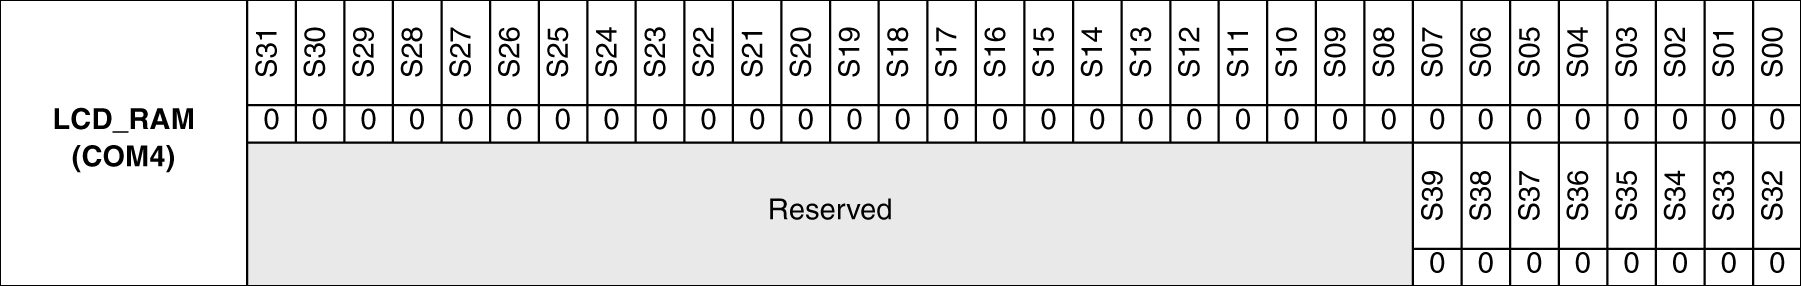
\includegraphics[scale=0.27]{Image/26.jpg}
\end{center}
\caption{Состав группы COM4}
\end{figure}

\begin{center}
\textit{В данной работе используется ЖКИ с 96 сегментами, разделенными на 4 группы COM0 -- COM3 по 24 сегмента каждая.}
\end{center}

\begin{figure}[h!]
\begin{center}
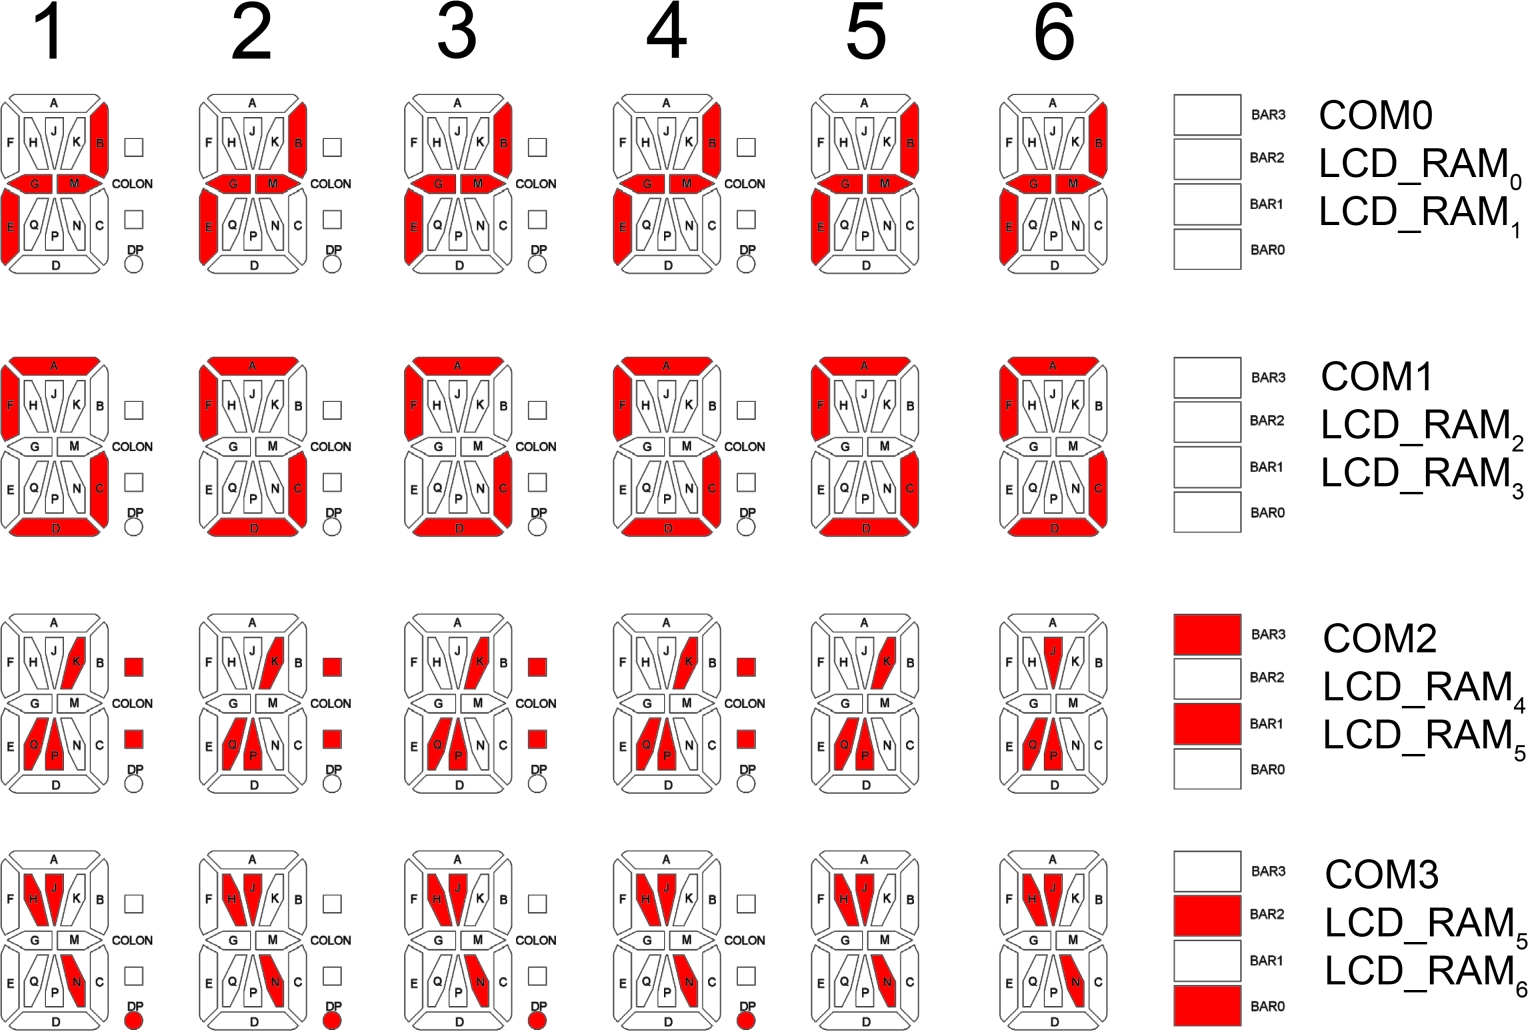
\includegraphics[scale=0.33]{Image/27.jpg}
\end{center}
\caption{Объединение сегментов в группы}\label{segment}
\end{figure}

ЖКИ на отладочной плате STM32L-Discovery подключен таким образом, что используются биты  \textit{S40, S41} вторых регистров \textit{LCD\_RAM} в каждой группе и биты  \textit{S0 -- S27} первых регистров \textit{LCD\_RAM}. Для уменьшения количества используемых регистров, информацию из битов  \textit{S40 --S43 }можно записывать в свободные биты  \textit{S28 -- S31}, используя \textit{функцию переназначения (remapping)}. 

\subsection{Блок делителей частоты}

Блок делителей частоты (Frequency generator) позволяет добиться различной частоты кадров (frame rates) на ЖКИ в диапазоне от 32 кГц до 1 МГц. В качестве источника тактирующего сигнала могут использоваться:
\begin{enumerate}
\item Внешний НЧ генератор с частотой 32 кГц (LSE. Low speed external).
\item Внутренний НЧ генератор с частотой 37 кГц (LSI. Low speed internal).
\item Внешний ВЧ генератор с делителями частоты на 2,4,8 и 16 и максимальной частотой 1 МГц. (HSE. High speed external)
\end{enumerate}

Для достижения точной синхронизации и снижения смещения напряжения постоянного тока через сегменты ЖКИ источник тактирующего сигнала должен обладать стабильностью. 

Тактирующий сигнал \textit{LCDCLK} поступает в контроллер ЖКИ. Частота тактового сигнала делится, в соответствии с коэффициентами деления, которые устанавливаются битами \textit{PS[3:0]}, \textit{DIV[3:0]} регистра \textit{LCD\_FCR }(Frame Control Register). Результирующая частота на выходе блока делителей частоты рассчитывается по формуле:


\[f_{ck\_div}=\frac{F_{LCDCLK}}{2^{PS}\cdot(16+DIV)}\]
Частота кадров рассчитывается по формуле:

\[ f_{Frame}=f_{ck\_div}\cdot duty\]
где $duty$ --- коэффициент заполнения -- отношение длительность импульса к его периоду. 

За время одного кадра на ЖКИ последовательно выводится информация из регистров \textit{LCD\_RAM[x]}, \textit{LCD\_RAM[x+1]} и тд. Для ЖКИ, установленного на отладочной плате, за один кадр, контроллер ЖКИ должен вывести информацию из 4 групп сегментов \textit{COM0 -- COM3}, следовательно, длительность управляющего импульса для одной группы будет 1/4 длительности кадра, т.е. \textit{duty=1/4}. 

\section{Динамическая и статическая индикация. Управление ЖКИ}

Существует два способа управления ЖКИ -- \textit{статический} режим управления и \textit{мультиплексный}\cite{gost25} режим управления. При статической индикации каждый сегмент разряда индикатора подключен к выходу микроконтроллера. Применительно к ЖКИ на отладочной плате STM32L-Discovery потребуется 6*14 = 84 выводов микроконтроллера (без учета двоеточий, точек и полосок). Из-за использования такого количества выводов, подключение другой периферии станет невозможным. Микроконтроллер STM32L152RB имеет 64 вывода.
	
	При мультиплексном режиме управлении (динамический режим управления) одинаковые сегменты разрядов индикатора объединены в группы. Отображение информации происходит за счет поочередного зажигания сегментов разрядов индикатора, с частотой, не воспринимаемой человеческим глазом. На рисунке \ref{t0} -- \ref{t3} условно изображен принцип работы динамической индикации. На ЖКИ выводится число 3114.


\begin{figure}[H]
\begin{center}
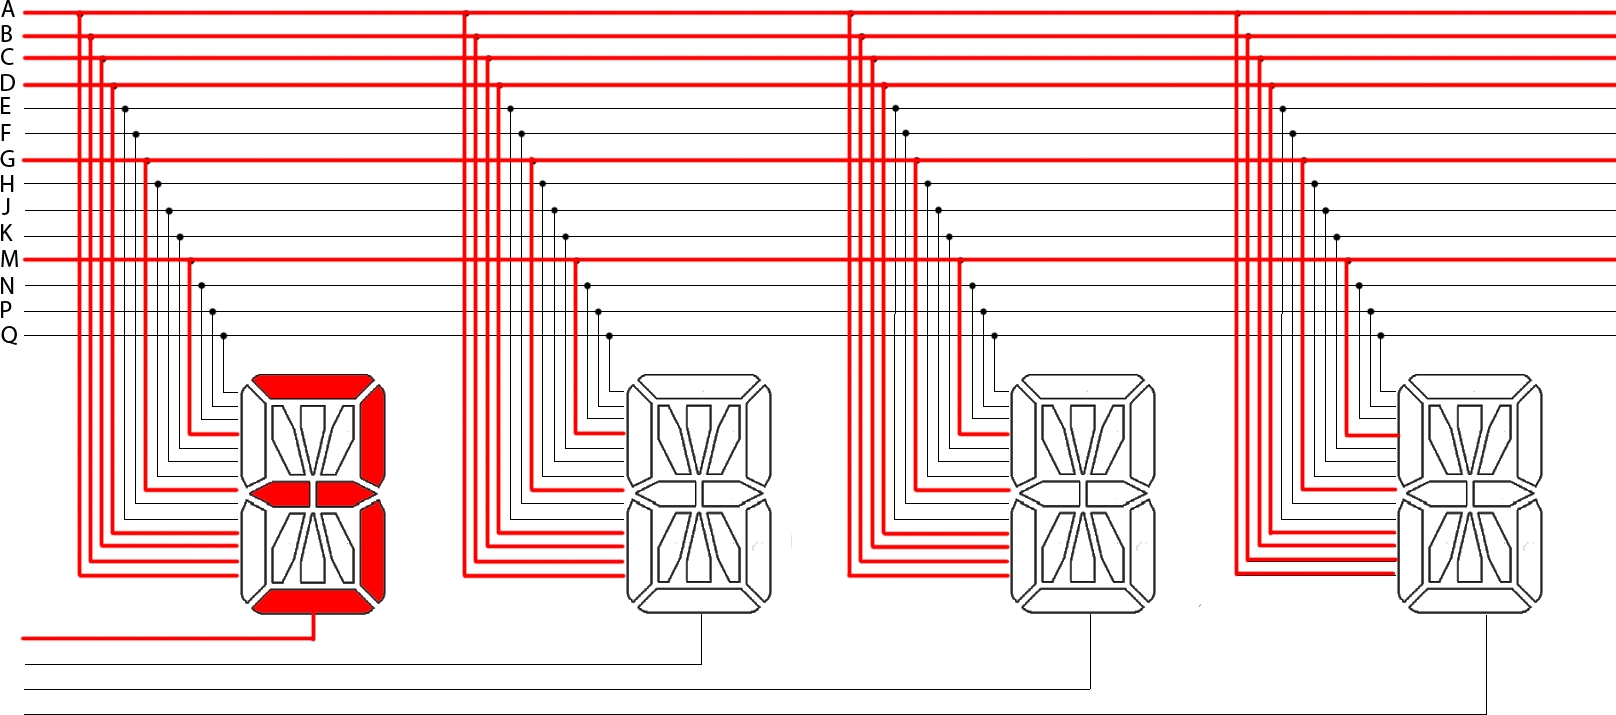
\includegraphics[scale=0.28]{Image/28.jpg} 
\end{center}
\caption{Работа ЖКИ в момент времени $t_0$}\label{t0}
\end{figure}

\begin{figure}[H]
\begin{center}
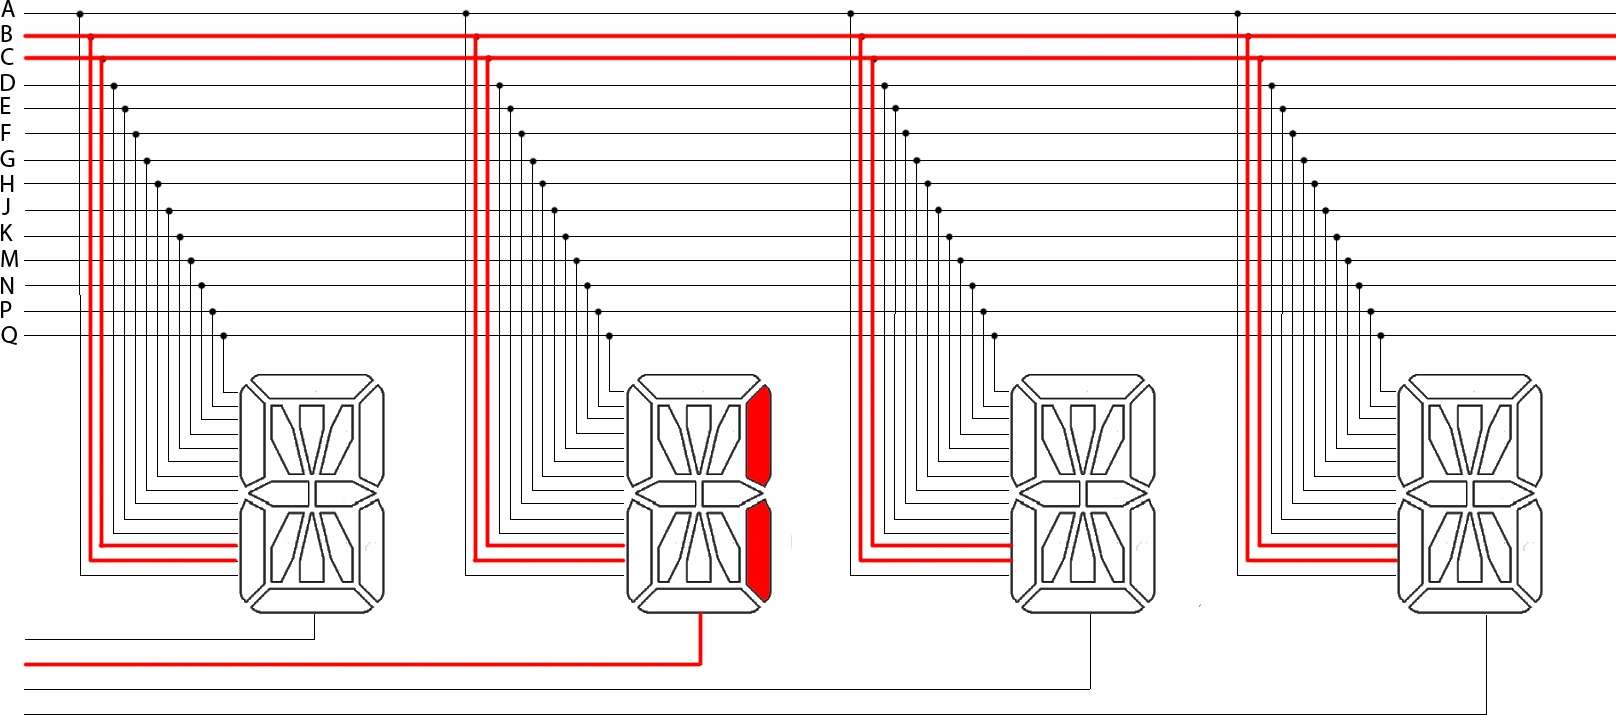
\includegraphics[scale=0.28]{Image/29.jpg}
\end{center}
\caption{Работа ЖКИ в момент времени $t_1$}
\end{figure}


\begin{figure}[H]
\begin{center}
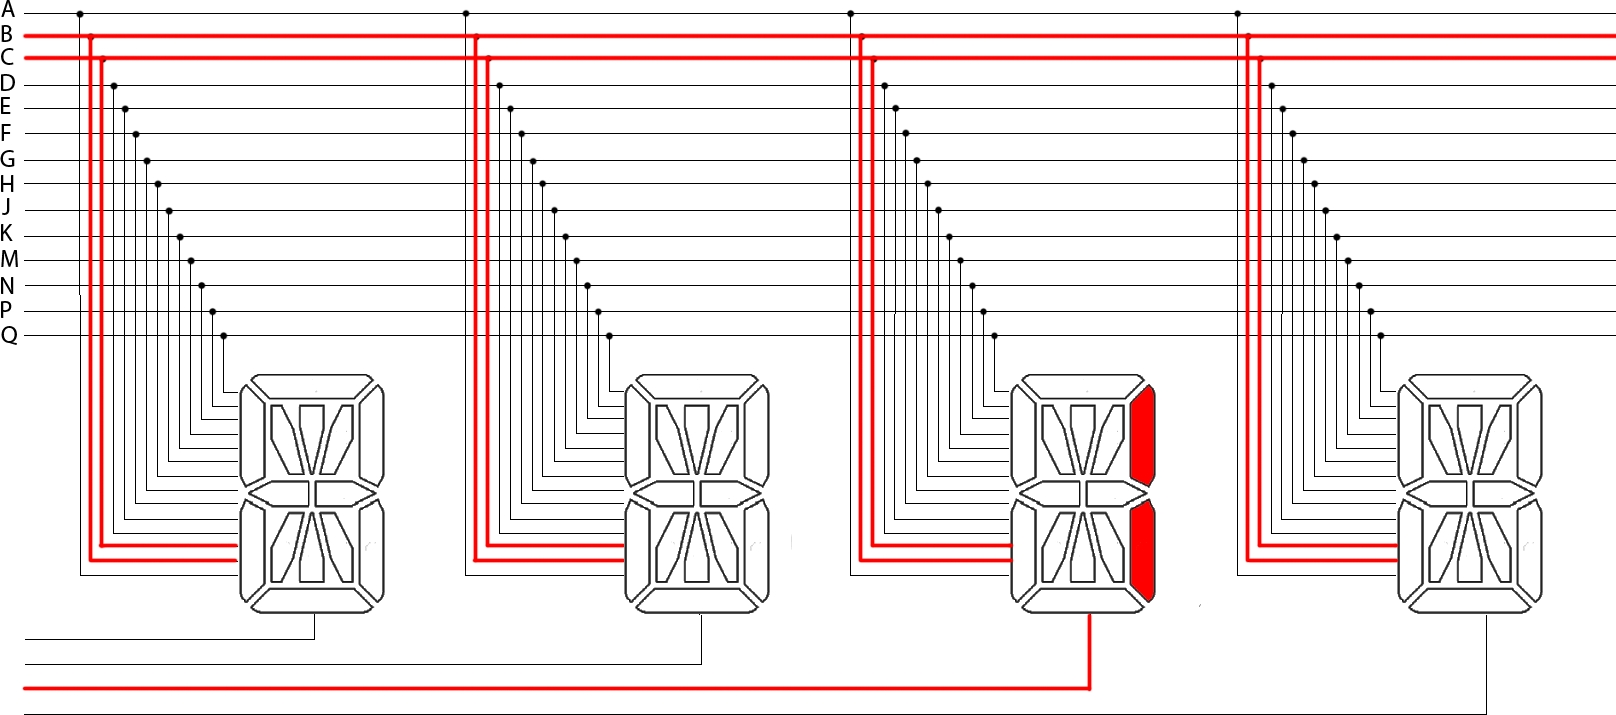
\includegraphics[scale=0.28]{Image/30.jpg}
\end{center}
\caption{Работа ЖКИ в момент времени $t_2$}
\end{figure}

\begin{figure}[H]
\begin{center}
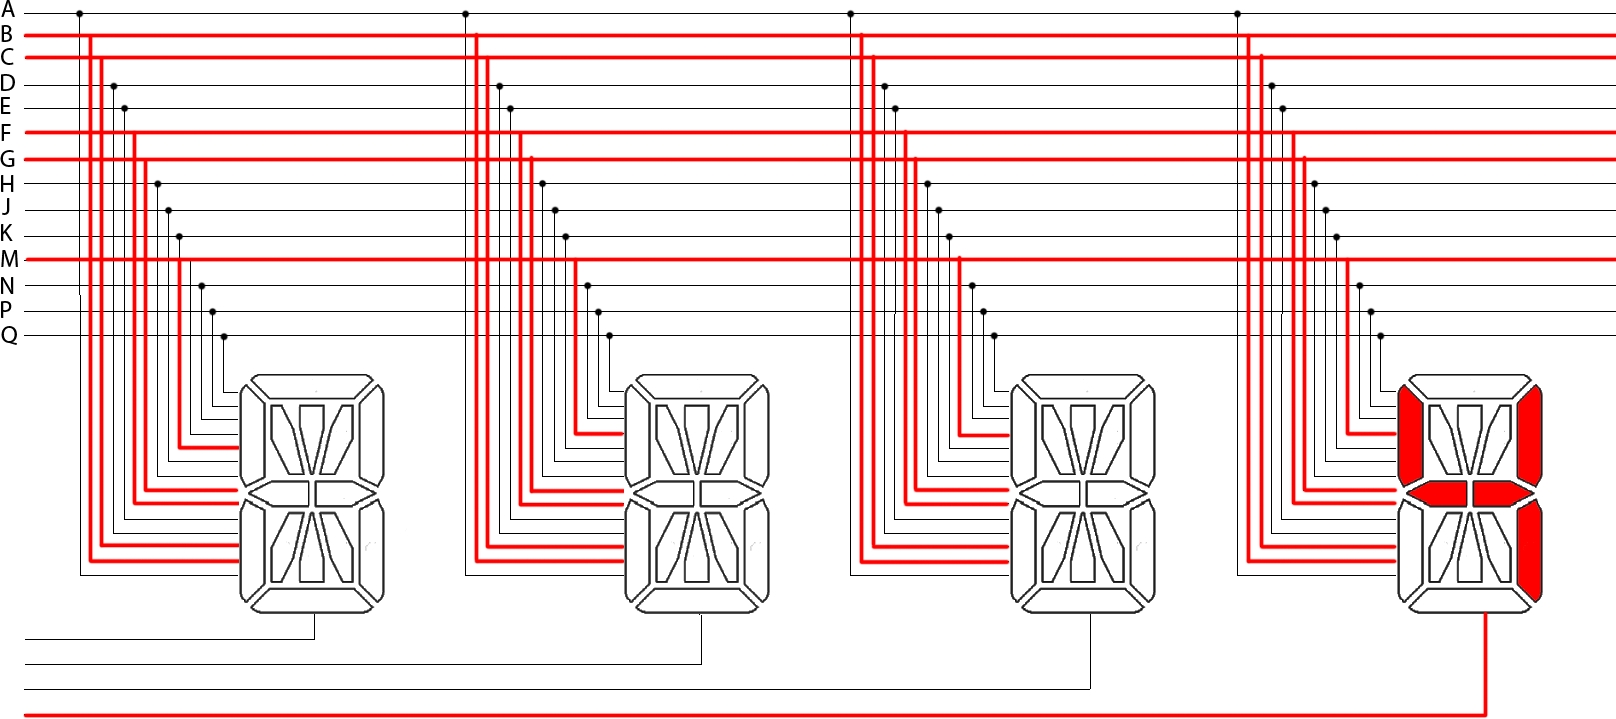
\includegraphics[scale=0.28]{Image/31.jpg} 
\end{center}
\caption{Работа ЖКИ в момент времени $t_3$}\label{t3}
\end{figure}

Мультиплексное управление позволяет управлять большим количеством сегментов. Вместо раздельного управления каждым элементом, они могу адресоваться по строкам и столбцам (COM и SEG (обозначение сегментов приведено на рисунке \ref{shema})), таким образом, упрощается управляющая схема, т.к. каждому сегменту не требуется собственная управляющая линия. Для включения выбранного сегмента, на него надо подать разность потенциалов \textit{COM} и \textit{SEG}. Пример работы первого разряда индикатора, используемого в данной работе, изображен на рисунке \ref{t01} -- \ref{t31}. На индикатор выводится <<1:>>.

\begin{figure}[H]
\begin{center}
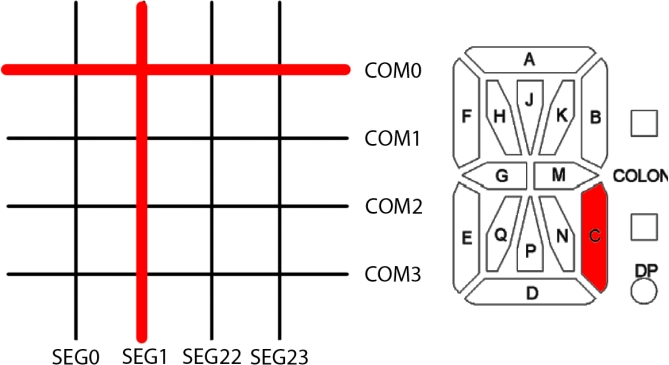
\includegraphics[scale=0.4]{Image/32.jpg} 
\end{center}
\caption{Первый разряд индикатора в момент времени $t_0$}\label{t01}
\end{figure}


\begin{figure}[H]
\begin{center}
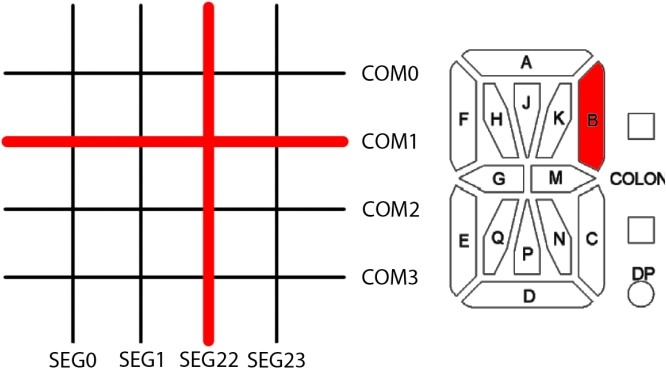
\includegraphics[scale=0.4]{Image/33.jpg} 
\end{center}
\caption{Первый разряд индикатора в момент времени $t_1$}
\end{figure}


\begin{figure}[H]
\begin{center}
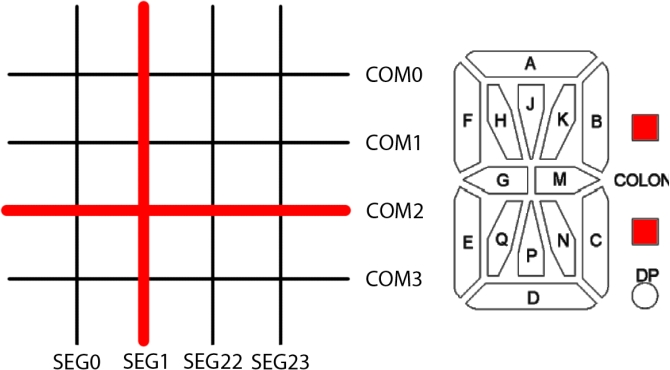
\includegraphics[scale=0.4]{Image/34.jpg} 
\end{center}
\caption{Первый разряд индикатора в момент времени $t_2$}\label{t31}
\end{figure}

Общая схема подключения сегментов к выводам ЖКИ \cite{scheme} приведена на рисунке \ref{shema}.


\begin{figure}[H]
\begin{center}
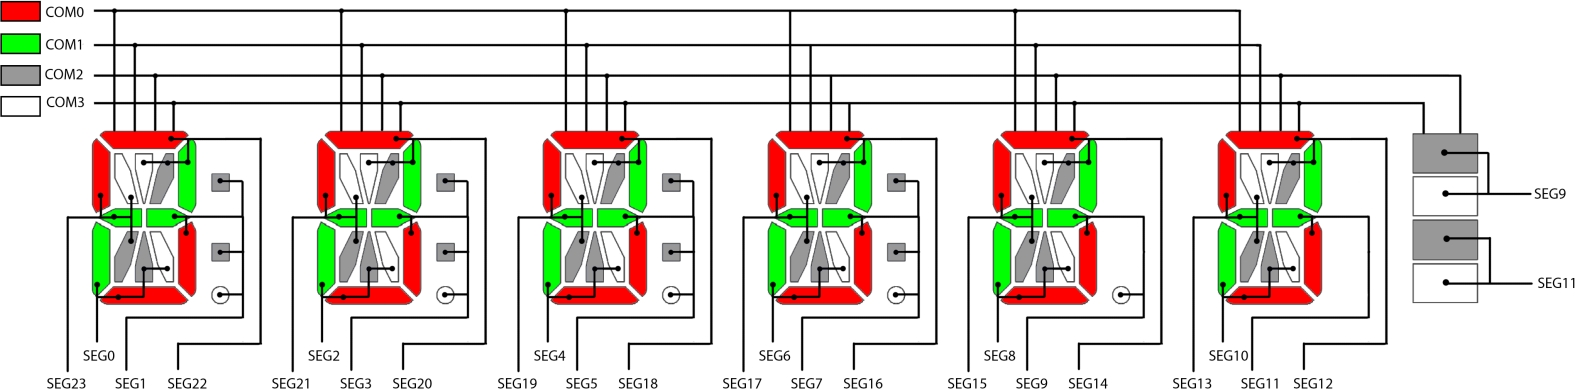
\includegraphics[scale=0.33]{Image/35.jpg} 
\end{center}
\caption{Схема подключения сегментов к выводам ЖКИ}\label{shema}
\end{figure}

Схема подключения выводов ЖКИ к портам микроконтроллера приведена на рисунке \ref{shema2}.


\begin{figure}[H]
\begin{center}
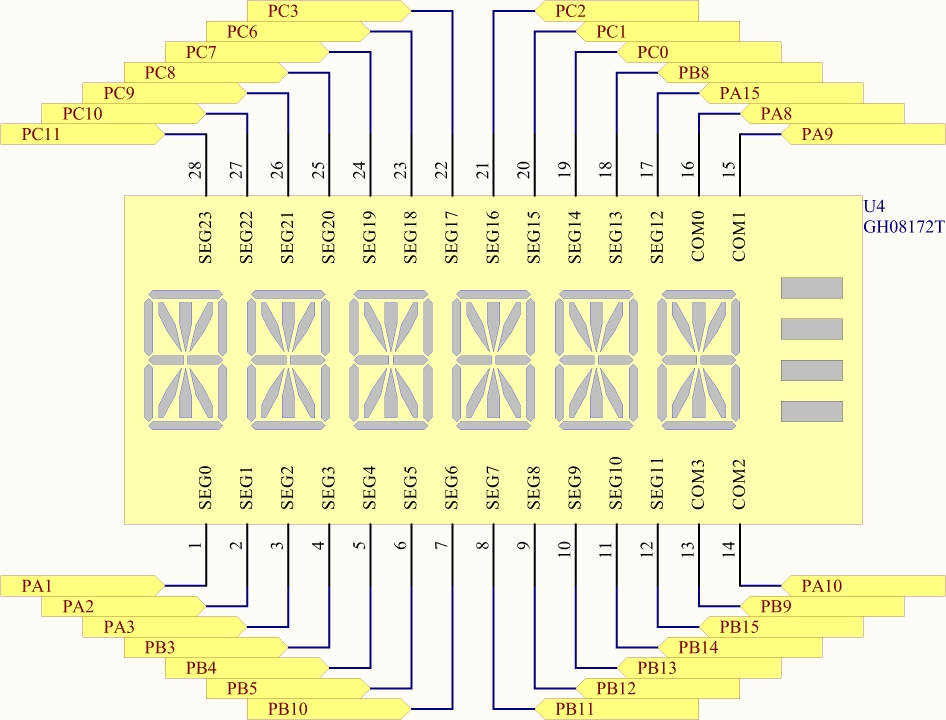
\includegraphics[scale=0.38]{Image/36.jpg} 
\end{center}
\caption{Схема подключения выводов ЖКИ к портам микроконтроллера}\label{shema2}
\end{figure}

Для линий \textit{SEG} используется управляющее напряжение, количество уровней которого определяется коэффициентом \textit{bias}. ЖКИ на отладочной плате использует мультиплексный режим управления с \textit{duty=1/4} и\textit{ bias=1/3}. Значение duty и bias устанавливаются через регистр \textit{LCD\_CR} (Control Register) в битах \textit{DUTY[2:0]} и\textit{ BIAS[1:0]}. Форма управляющих напряжений для \textit{duty=1/4} и \textit{bias=1/3} приведена на рисунке \ref{pit}.

\begin{figure}[H]
\begin{center}
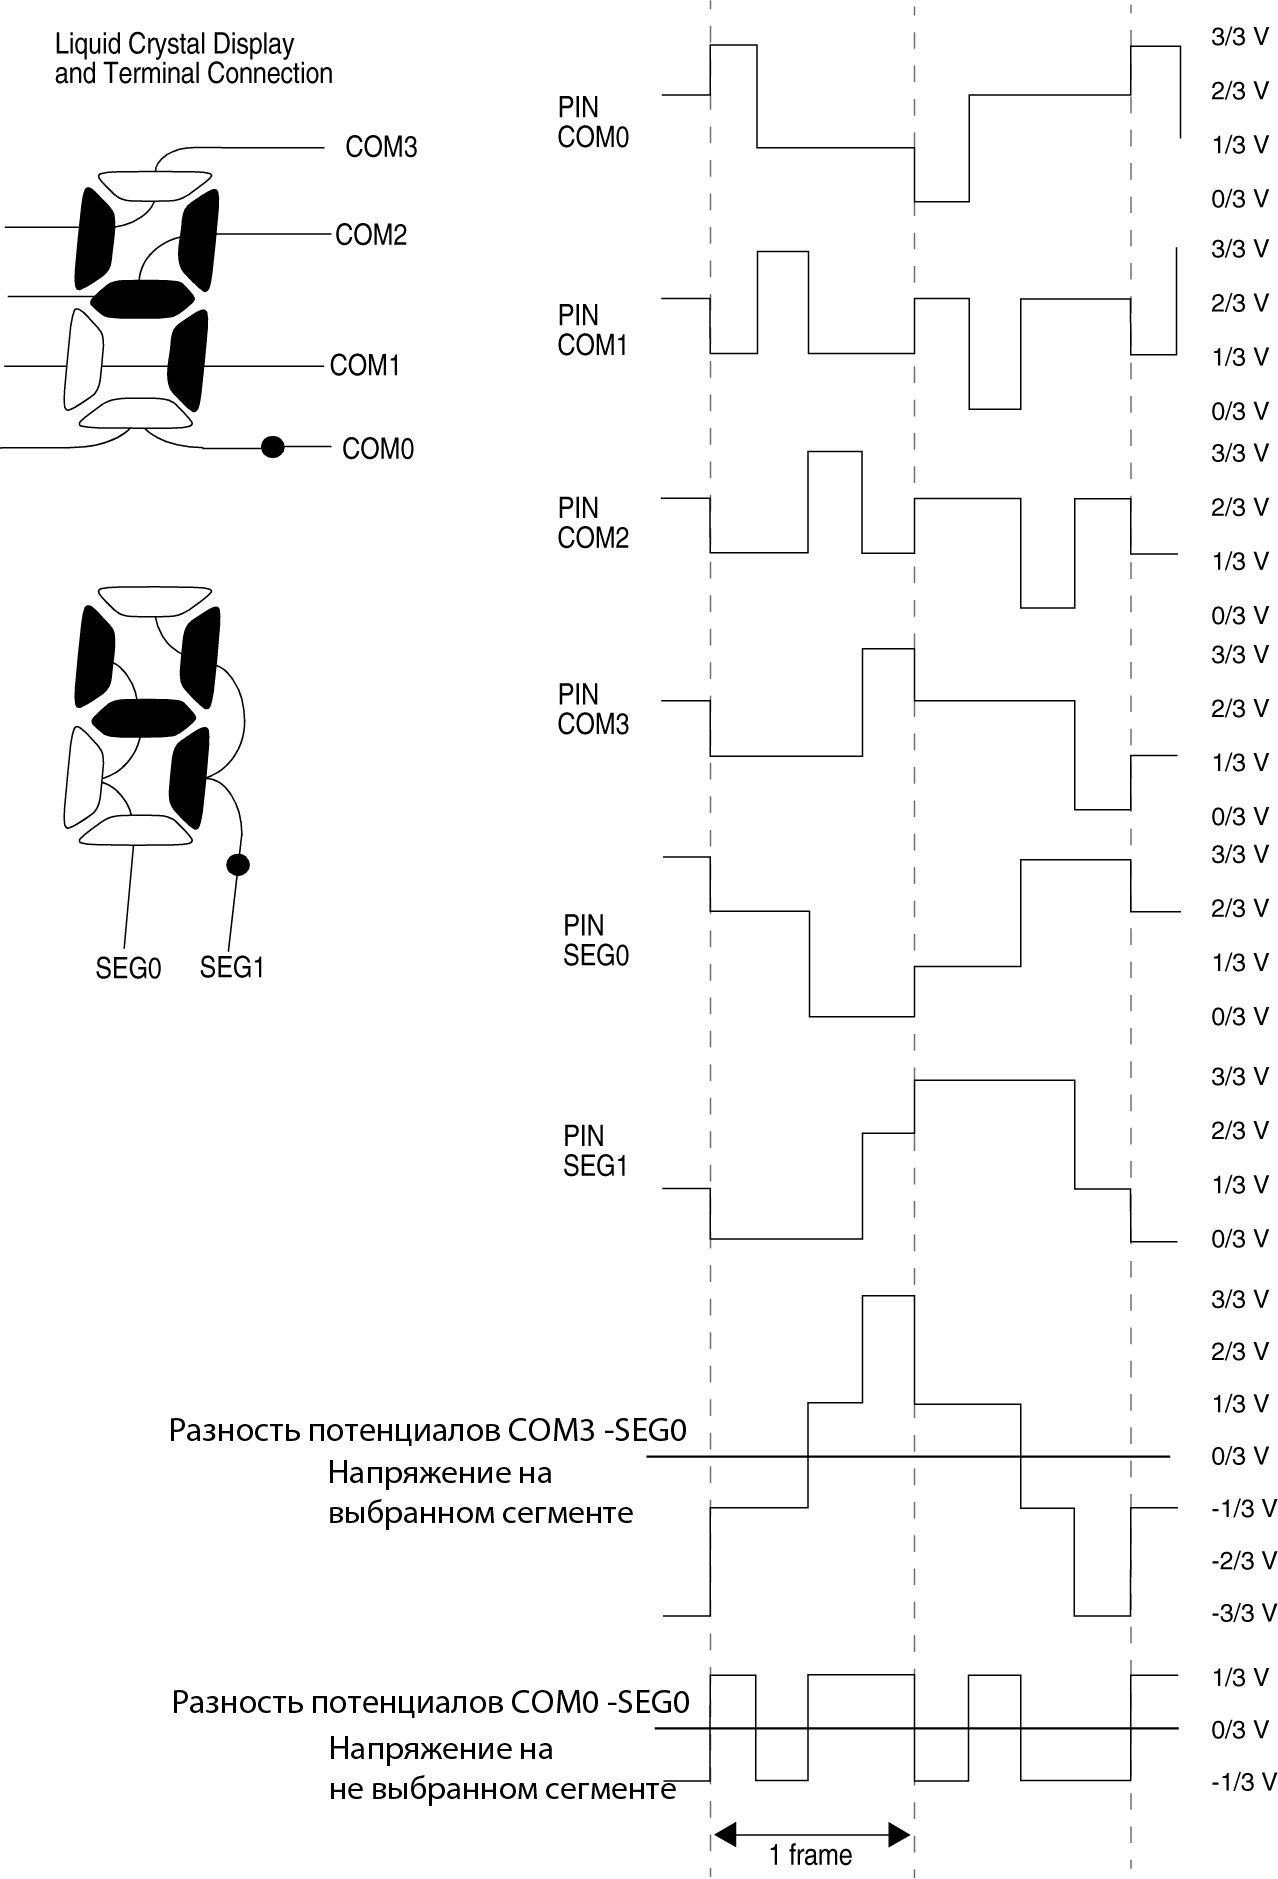
\includegraphics[scale=0.33]{Image/37.jpg} 
\end{center}
\caption{Форма управляющих сигналов}\label{pit}
\end{figure}

\section{Конфигурирование микроконтроллера}
\subsection{Регистры периферии. Запись в регистры}

Для управления ЖКИ порты микроконтроллера должны быть настроены соответствующим образом:
\begin{enumerate}
\item На выход.
\item Использование альтернативной функции \textit{AF 11} (Alternate function).
\item Иметь частоты вывода в порт 400 кГц.
\item Использовать режим работы \textit{push -- pull}.
\item Без подтягивающих резисторов. 
\end{enumerate}


При работе порта в режиме альтернативной функции, выходной буфер данных порта управляется сигналами, поступающими с периферии. Заголовочный файл \textit{stm32l1xx.h} библиотеки CMSIS содержит описание всех регистров периферии, объединенных в структуры:
\begin{verbatim}
...
typedef struct
{
  __IO uint32_t MODER;
  __IO uint16_t OTYPER;
  uint16_t RESERVED0;
  __IO uint32_t OSPEEDR;
  __IO uint32_t PUPDR;
  __IO uint16_t IDR;
  uint16_t RESERVED1;
  __IO uint16_t ODR;
  uint16_t RESERVED2;
  __IO uint16_t BSRRL; /* BSRR register is split to 
                    		  2 * 16-bit fields BSRRL 
  __IO uint16_t BSRRH; /* BSRR register is split to 
                       2 * 16-bit fields BSRRH 
  __IO uint32_t LCKR;
  __IO uint32_t AFR[2];
} GPIO_TypeDef;
...
typedef struct
{
  __IO uint32_t CR;
  __IO uint32_t ICSCR;
  __IO uint32_t CFGR;
  __IO uint32_t CIR;
  __IO uint32_t AHBRSTR;
  __IO uint32_t APB2RSTR;
  __IO uint32_t APB1RSTR;
  __IO uint32_t AHBENR;
  __IO uint32_t APB2ENR;
  __IO uint32_t APB1ENR;
  __IO uint32_t AHBLPENR;
  __IO uint32_t APB2LPENR;
  __IO uint32_t APB1LPENR;      
  __IO uint32_t CSR;    
} RCC_TypeDef;
...
\end{verbatim}
Для удобного обращения определены константы:
\begin{verbatim}
...
#define RCC                 ((RCC_TypeDef *) RCC_BASE)
#define CRC                 ((CRC_TypeDef *) CRC_BASE)
...
#define GPIOA               ((GPIO_TypeDef *) GPIOA_BASE)
#define GPIOB               ((GPIO_TypeDef *) GPIOB_BASE)
#define GPIOC               ((GPIO_TypeDef *) GPIOC_BASE)
#define GPIOD               ((GPIO_TypeDef *) GPIOD_BASE)
#define GPIOE               ((GPIO_TypeDef *) GPIOE_BASE)
#define GPIOH               ((GPIO_TypeDef *) GPIOH_BASE)
...

\end{verbatim}

Определенные таким образом структуры и указатели используются для доступа к конкретным регистрам периферии. Пример записи значения в регистр \textit{MODER} порта \textit{GPIOA}:
\begin{verbatim}
GPIOA->MODER = 0x4;
\end{verbatim}
Пример записи значения в регистр \textit{AHBENR }системы тактирования и сброса \textit{RCC}:

\begin{verbatim}
RCC->AHBENR = 0x7;
\end{verbatim}
Для упрощения записи значений в регистры, в файле \verb\stm32lxx.h\, заранее определены битмаски --- расшифровка отдельных битов регистров по функциям. Вместо использования шестнадцатеричных значений используются заранее определенные константы.

\begin{verbatim}
...
#define GPIO_MODER_MODER1          ((uint32_t)0x0000000C)
#define GPIO_MODER_MODER1_0        ((uint32_t)0x00000004)
#define GPIO_MODER_MODER1_1        ((uint32_t)0x00000008)
#define GPIO_MODER_MODER2          ((uint32_t)0x00000030)
...
\end{verbatim}
Пример записи значения в регистр \textit{MODER} порта \textit{GPIOA}:
\begin{verbatim}
GPIOA->MODER |= GPIO_MODER_MODER1_0;
\end{verbatim}
Результат выполнения строки аналогичен \verb#GPIOA->MODER = 0x4#;

%%%%%%%%%%%%%%%%%%%%%%%%%%%%%%%%%%%%%%%%%%%%


%Дописать


%%%%%%%%%%%%%%%%%%%%%%%%%%%%%%%%%%%%%%%%%%%
\subsection{Конфигурирование портов микроконтроллера}

Выводы ЖКИ подключены к портам \textit{GPIOA} (PA1 -- PA3, PA8 -- PA10, PA15), \textit{GPIOB} (PB3 -- PB5, PB8 -- PB15), \textit{GPIOC} (PC0 -- PC3, PC6 -- PC11) микроконтроллера. (см. рисунок \ref{shema2}). Для работы ЖКИ на выбранные порты необходимо подать тактовый сигнал. Тактирование портов\textit{ GPIO} микроконтроллера происходит от шины \textit{AHB} системы \textit{RCC} (Reset and Clock Control) -- системы тактировании и сброса. Подача тактового сигнала осуществляется установкой соответствующих битов в регистре \textit{RCC\_AHBENR} (AHB peripheral clock enable register). 


\begin{figure}[H]
\begin{center}
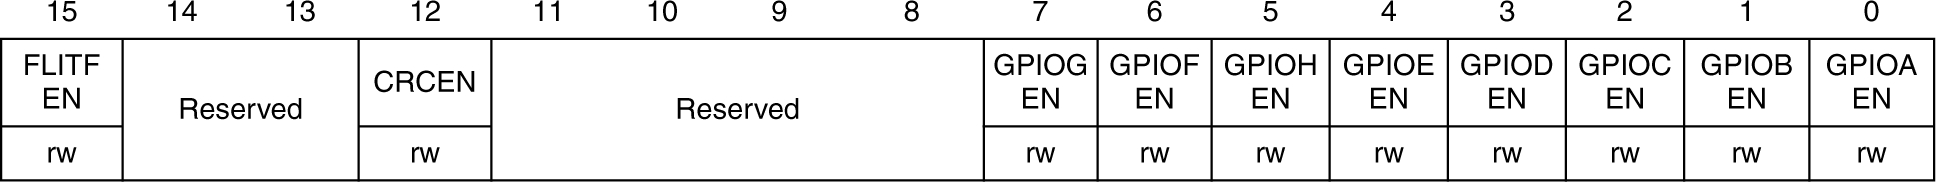
\includegraphics[scale=0.25]{Image/38.jpg} 
\end{center}
\caption{Регистр \textit{RCC\_AHBENR} (приведены первые 15 разрядов)}
\end{figure}

Для портов \textit{GPIOA, GPIOB, GPIOC} необходимо установить \verb\1\ в 0, 1, 2 разряды регистра. 

\begin{verbatim}
RCC->AHBENR |= (RCC_AHBENR_GPIOAEN | RCC_AHBENR_GPIOBEN
                | RCC_AHBENR_GPIOCEN)
                
// RCC->AHBENR = 0x7; 
// 0x7 = 111
\end{verbatim}

	Для указания режимов работы порта используется регистр \textit{GPIOx\_MODER} (GPIO port mode register) (x = A \ldots H). Все разряды регистра сгруппированы в группы \textit{MODERy[1:0]}, где y номер пина соответствующего порта. Порты необходимо настроить на режим альтернативной функции, т.е. в группе, отвечающей за пин, установить значение \verb\10\. Для порта \textit{GPIOA }нужно настроить пины 1 -- 3, 8 -- 10, 15, т.е установить \verb\1\ в 3, 5, 7, 17, 19, 21, 31 разряды. 


\begin{figure}[H]
\begin{center}
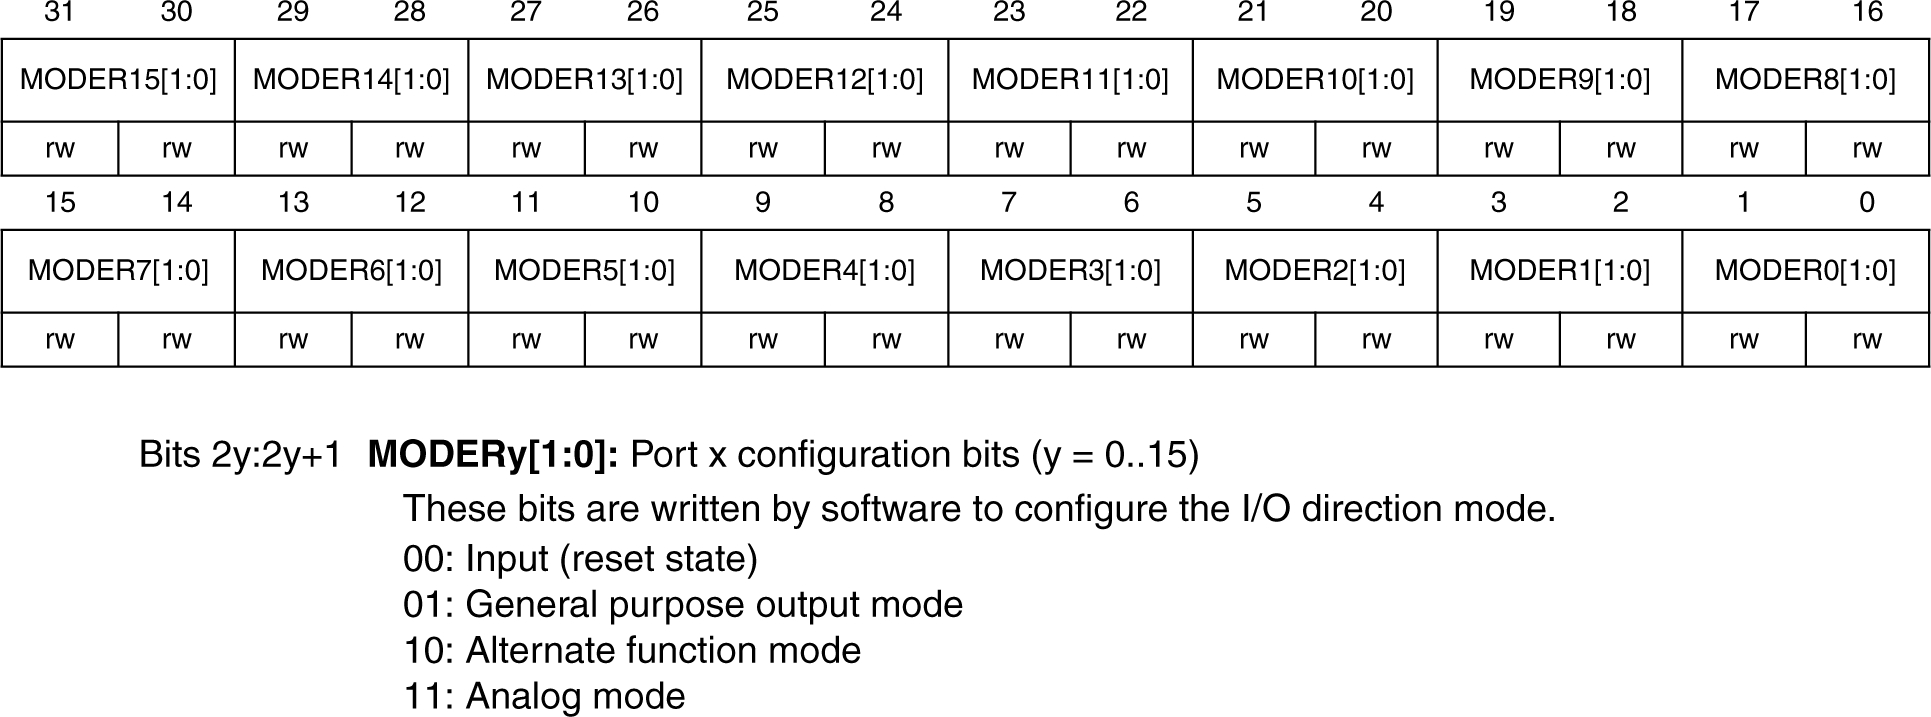
\includegraphics[scale=0.25]{Image/39.jpg} 
\end{center}
\caption{Регистр \textit{GPIOx\_MODER} (GPIO port mode register)}
\end{figure}
\begin{verbatim}
GPIOA->MODER |= (GPIO_MODER_MODER1_1 | GPIO_MODER_MODER2_1 
               | GPIO_MODER_MODER3_1 | GPIO_MODER_MODER8_1 |
                 GPIO_MODER_MODER9_1 | GPIO_MODER_MODER10_1 | 
                 GPIO_MODER_MODER15_1);

// GPIOA->MODER = 0x802A00A8;
// 0x802A00A8 = 1000 0000 0010 1010 0000 0000 1010 1000 
\end{verbatim}


Порты микроконтроллера необходимо перевести в режим \textit{push -- pull}. Для этого необходимо в регистре \textit{GPIOx\_OTYPER} (GPIO port output type register) установить \verb\1\ в разряды, отвечающие за пины. 
\begin{figure}[H]
\begin{center}
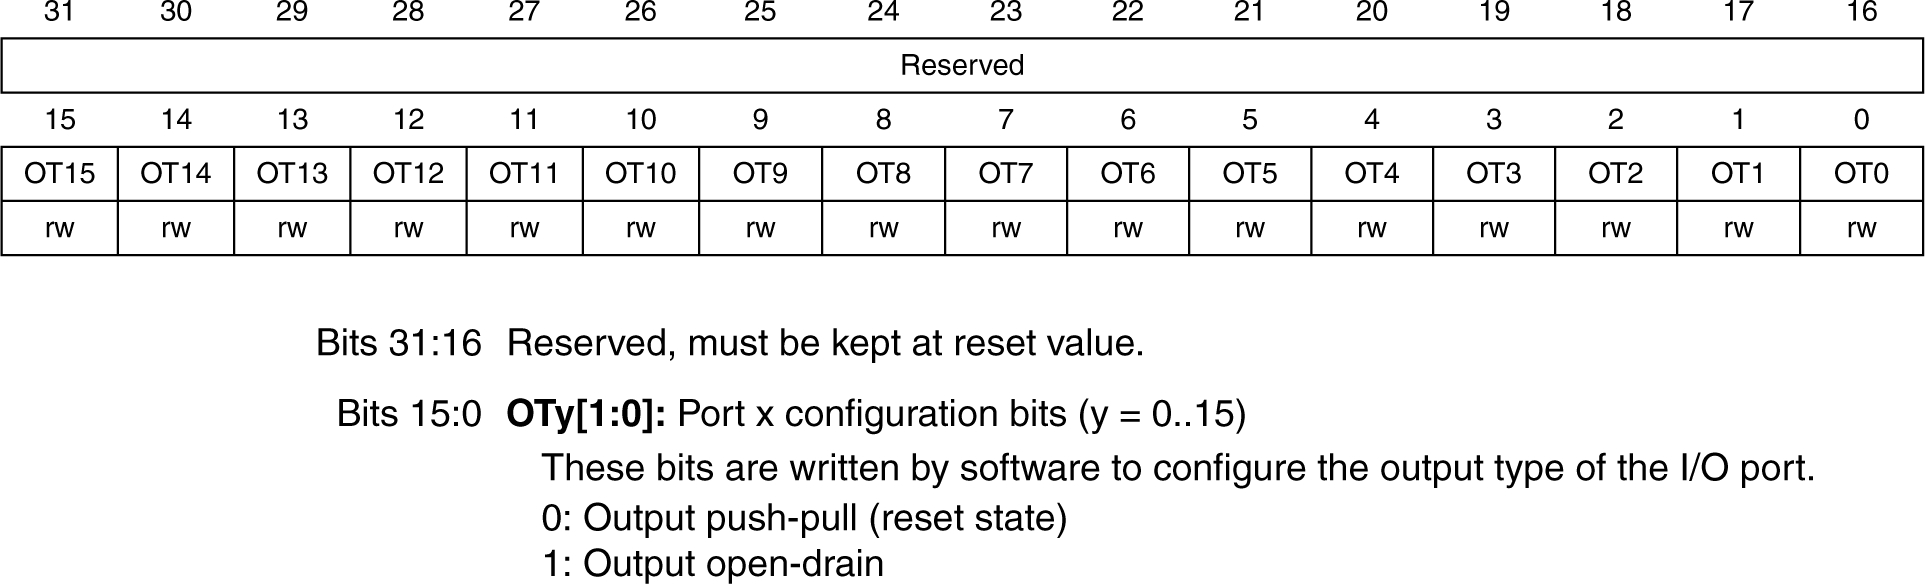
\includegraphics[scale=0.25]{Image/40.jpg} 
\end{center}
\caption{Регистр \textit{GPIOx\_OTYPER} (GPIO port output type register)}
\end{figure}

\begin{verbatim}
GPIOA->OTYPER &= ~(GPIO_OTYPER_OT_1 | GPIO_OTYPER_OT_2 |
                   GPIO_OTYPER_OT_3 | GPIO_OTYPER_OT_8 | 
                   GPIO_OTYPER_OT_9 | GPIO_OTYPER_OT_10 |
                   GPIO_OTYPER_OT_15);

// GPIOA->OTYPER &= ~0x0000870E;
// 0x870E = 1000 0111 0000 1110 
\end{verbatim}

Оба варианта воздействуют на выбранные пины. (Для порта GPIOA настраиваются пины 1 -- 3, 8 -- 10, 15). Если необходимо перевести все пины порта в режим \textit{push -- pull}, можно записать в регистр значение:

\begin{verbatim}
GPIOA->OTYPER = 0x0;
\end{verbatim}


Для указания частоты вывода информации в порт используется регистр \textit{ GPIOx\_OSPEEDR} (GPIO port output speed register). Все разряды регистра сгруппированы в группы \textit{OSPEEDRy[1:0]}, где y номер пина соответствующего порта. В данной работе должна быть установлена частота 400 кГц т.е. в группе, отвечающей за пин, установить значение \verb\00\. 


\begin{figure}[H]
\begin{center}
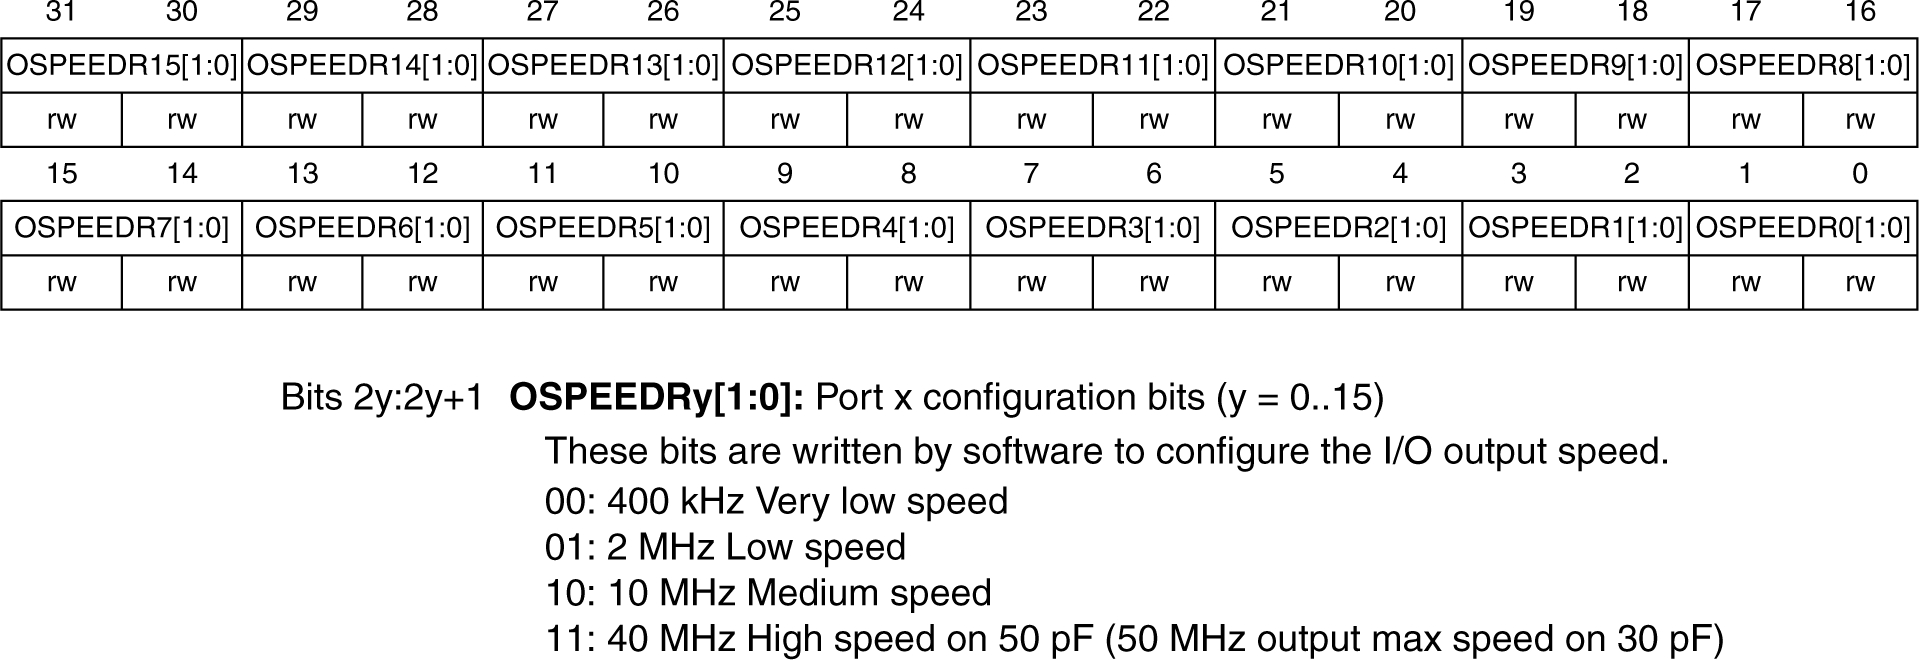
\includegraphics[scale=0.25]{Image/41.jpg} 
\end{center}
\caption{Регистр \textit{ GPIOx\_OSPEEDR} (GPIO port output speed register)}
\end{figure}

\begin{verbatim}
GPIOA->OSPEEDR &= ~(GPIO_OSPEEDER_OSPEEDR1 | GPIO_OSPEEDER_OSPEEDR2 |
                    GPIO_OSPEEDER_OSPEEDR3 | GPIO_OSPEEDER_OSPEEDR8 | 
                    GPIO_OSPEEDER_OSPEEDR9 | GPIO_OSPEEDER_OSPEEDR10 | 
                    GPIO_OSPEEDER_OSPEEDR15);

// GPIOA->OSPEEDR &= ~0xC03F00FC;
// 0xC03F00FC = 1100 0000 0011 1111 0000 0000 1111 1100 
\end{verbatim}
Если необходимо установить частоту вывода в порт 400 кГц для всех пинов, можно записать в регистр значение:
\begin{verbatim}
GPIOA->OSPEEDR = 0x0;
\end{verbatim}

Для отключения подтягивающих резисторов \textit{pull-up, pull-down} для выбранных пинов используется регистр \textit{GPIOx\_PUPDR }(GPIO port pull-up/pull-down register). Все разряды регистра сгруппированы в группы \textit{PUPDRy[1:0]}, где \textit{y} -- номер пина соответствующего порта. Для отключение подтягивающих резисторов в группе, отвечающей за пин, устанавливается значение \verb\00\. 

\begin{figure}[H]
\begin{center}
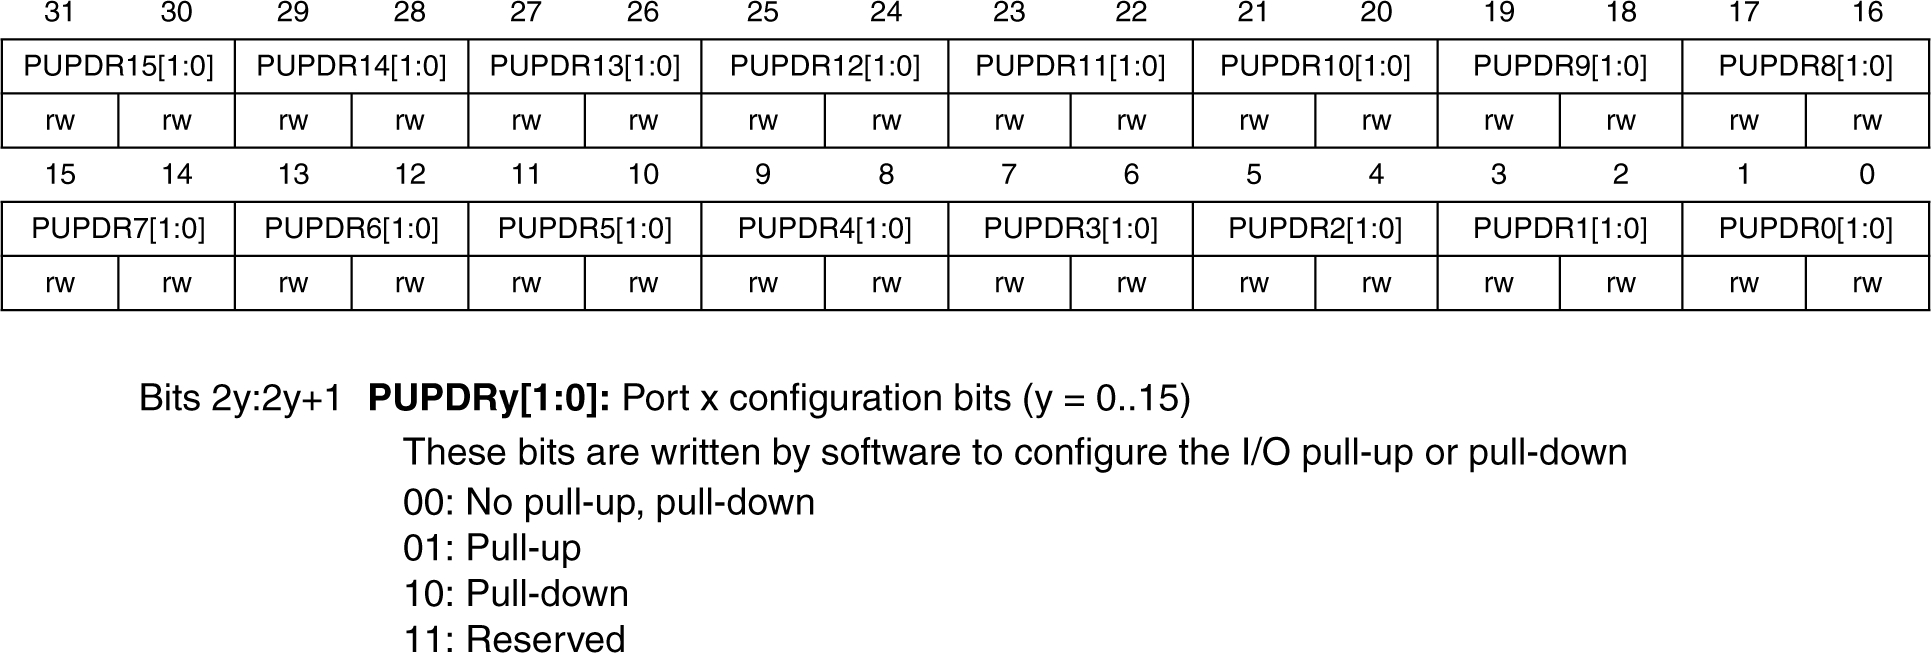
\includegraphics[scale=0.25]{Image/42.jpg} 
\end{center}
\caption{Регистр \textit{GPIOx\_PUPDR }(GPIO port pull-up/pull-down register)}
\end{figure}

\begin{verbatim}
GPIOA->PUPDR &= ~(GPIO_PUPDR_PUPDR1 | GPIO_PUPDR_PUPDR2 |
                  GPIO_PUPDR_PUPDR3 | GPIO_PUPDR_PUPDR8 | 
                  GPIO_PUPDR_PUPDR9 | GPIO_PUPDR_PUPDR10 | 
                  GPIO_PUPDR_PUPDR15);

// GPIOA->PUPDR &= ~0xC03F00FC;
// 0xC03F00FC = 1100 0000 0011 1111 0000 0000 1111 1100 
\end{verbatim}
Если необходимо отключить подтягивающие резисторы для всех пинов, можно записать в регистр значение:
\begin{verbatim}
GPIOA->PUPDR = 0x0;
\end{verbatim}

Для установки альтернативной функции для портов микроконтроллера используются два регистра \textit{GPIOx\_AFRL} (GPIO alternate function low register), отвечающий за младшие пины (с 0 по 7) и \textit{GPIOx\_AFRH} (GPIO alternate function high register), отвечающий за старшие пины (с 8 по 15). Все разряды регистров сгруппированы в группы \textit{AFRLy[3:0]} и \textit{AFRHy[3:0]}, где \textit{y} -- номер пина соответствующего порта. Порты должны быть настроены на использование альтернативной функции \textit{AF11}, для этого в группе, отвечающей за пин, должно быть установлено значение \verb\1011\.


\begin{figure}[H]
\begin{center}
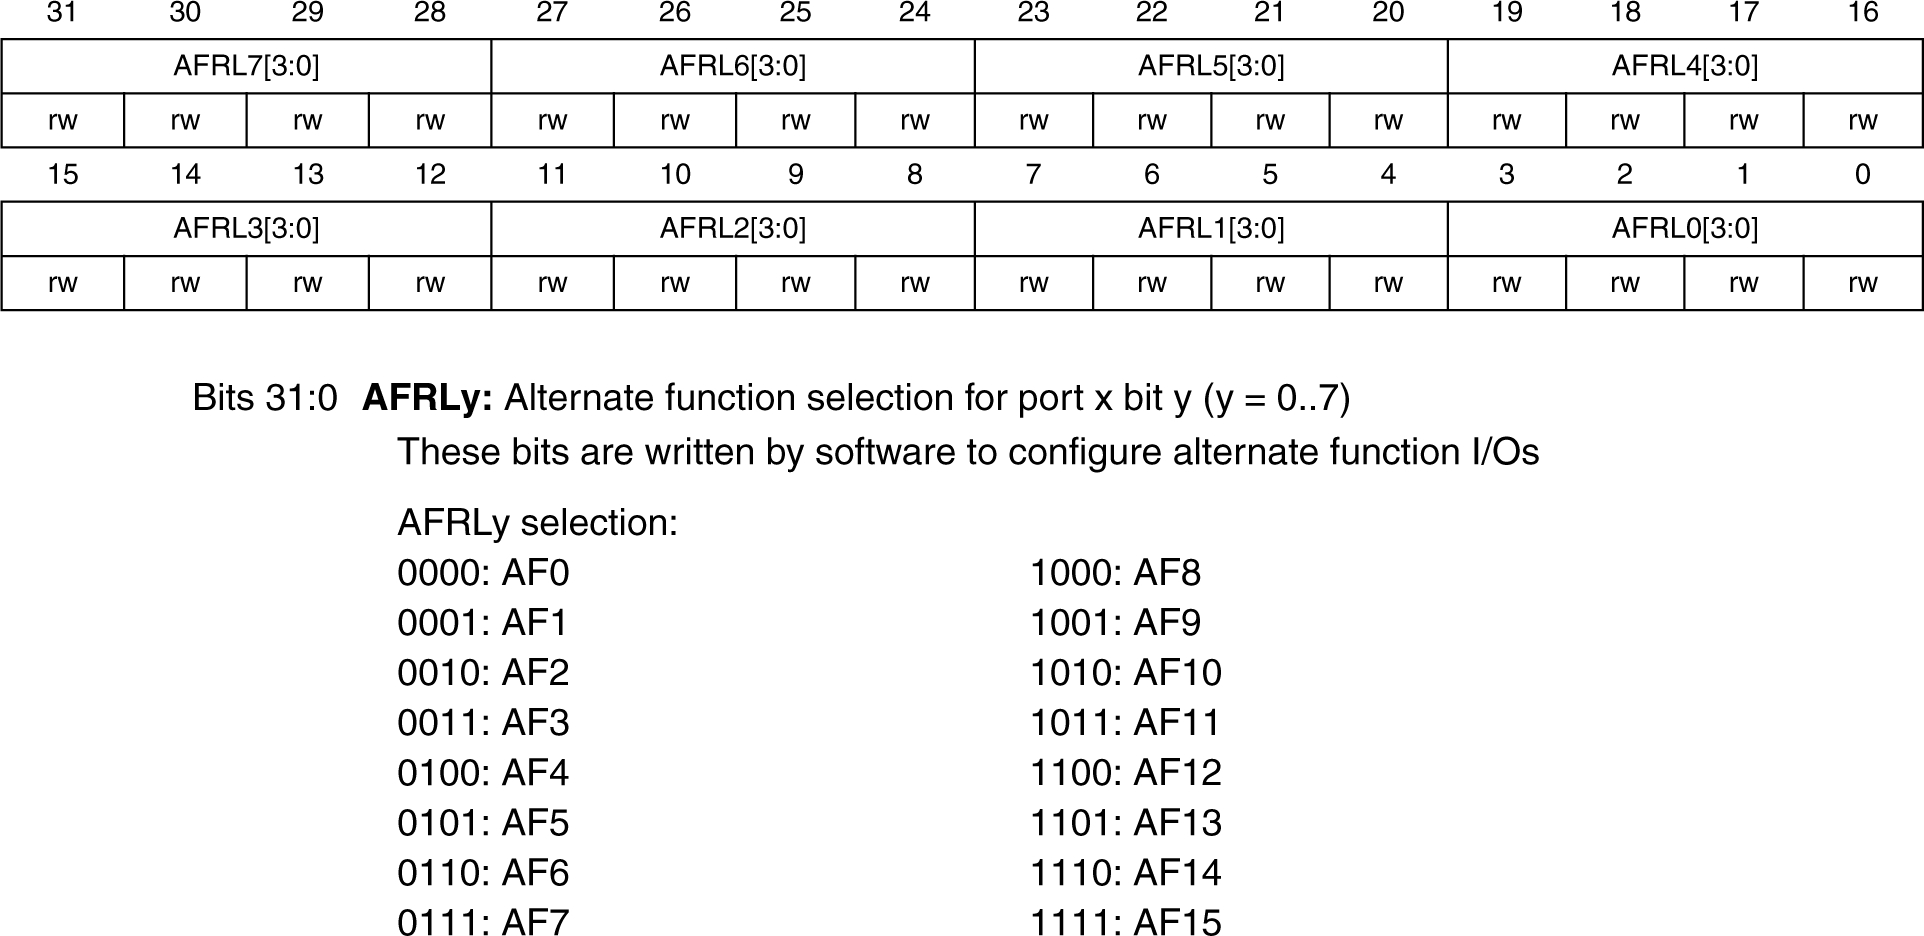
\includegraphics[scale=0.25]{Image/43.jpg} 
\end{center}
\caption{Регистр \textit{GPIOx\_AFRL} (GPIO alternate function low register)}
\end{figure}
\begin{figure}[H]
\begin{center}
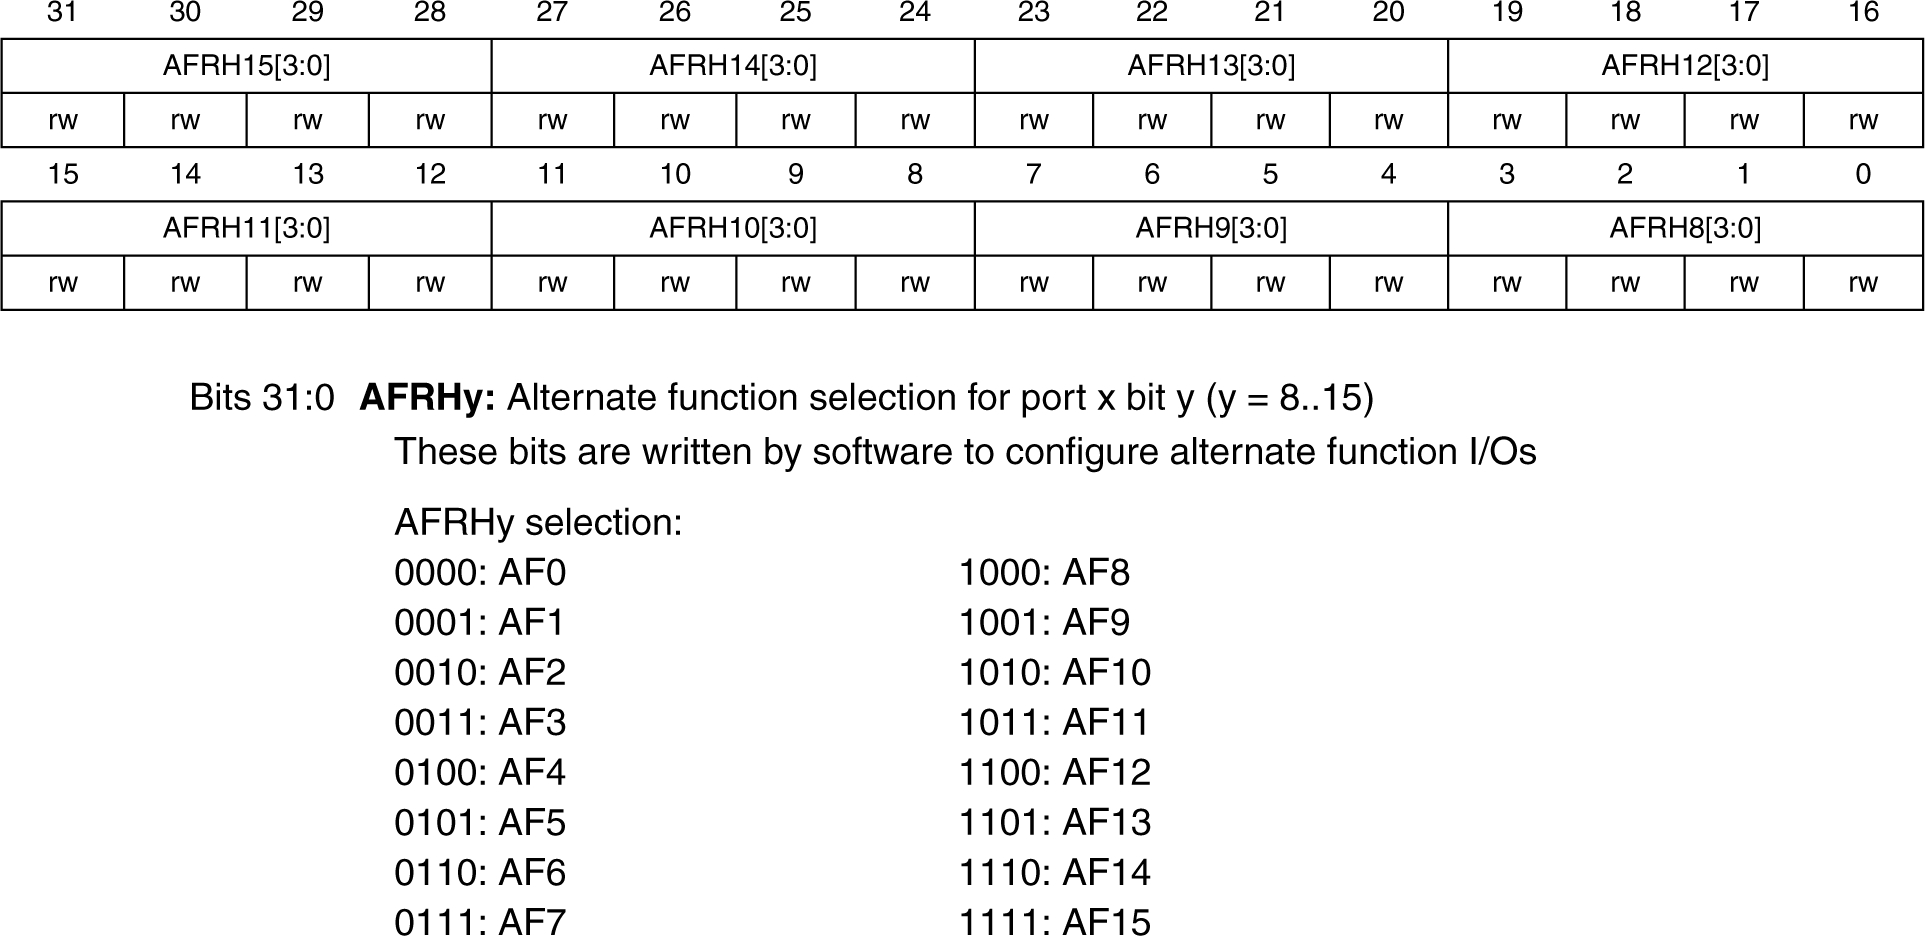
\includegraphics[scale=0.25]{Image/44.jpg} 
\end{center}
\caption{Регистр \textit{GPIOx\_AFRH} (GPIO alternate function high register)}
\end{figure}
Для этого необходимо записать в регистры значения:
\begin{verbatim}
GPIOA->AFR[0] = 0xBBB0;
// 0xBBB0 = 1011 1011 1011 0000_2 

GPIOA->AFR[1] = 0xB0000BBB;
// 0xB0000BBB = 1011 0000 0000 0000 0000 1011 1011 1011 
\end{verbatim}
\verb#AFR[0] = 0xBBB0# --- записывает значение в регистр \textit{GPIOx\_AFRL}.
\verb#AFR[1] = 0xB0000BBB# --- записывает значение в регистр \textit{GPIOx\_AFRH}.

Настройки соответствующих пинов портов \textit{GPIOB, GPIOC} производятся аналогично. Схема конфигурации порта приведена на рисунке \ref{portconf}. 

\begin{figure}[H]
\begin{center}
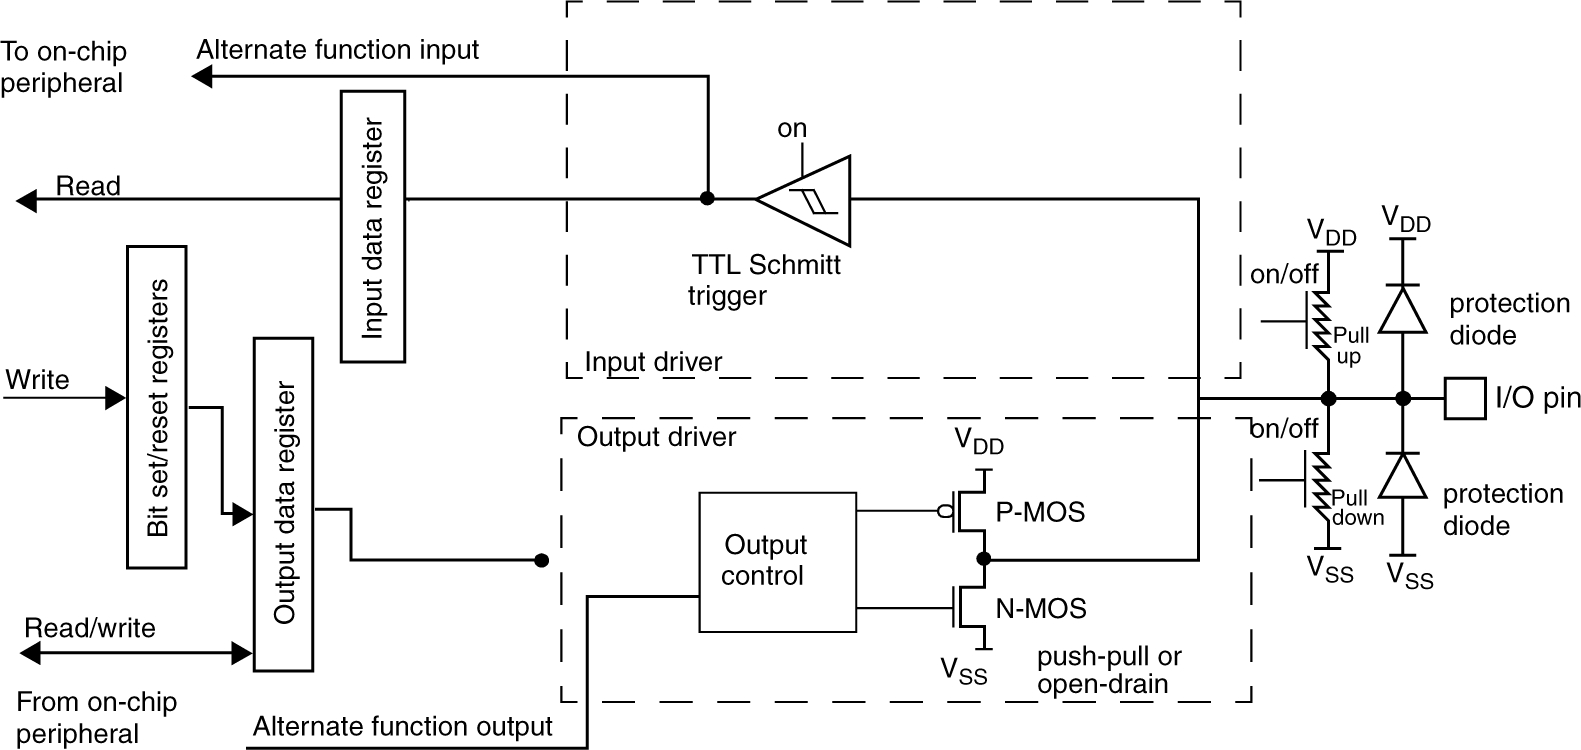
\includegraphics[scale=0.32]{Image/45.jpg} 
\end{center}
\caption{Схема конфигурации порта}\label{portconf}
\end{figure}


\section{Настройка контроллера ЖКИ}
При работе с контроллером ЖКИ, как и с другой периферией, на него необходимо подать тактовый сигнал. Тактовый сигнал также подается на систему управления питанием. Контроллер и система управления питанием для тактирования используют шину \textit{APB1}. Для разрешения тактирования в регистре \textit{RCC\_APB1ENR} (APB1 peripheral clock enable register) необходимо установить \verb\1\ в 9 и 28 разрядах.

\begin{figure}[H]
\begin{center}
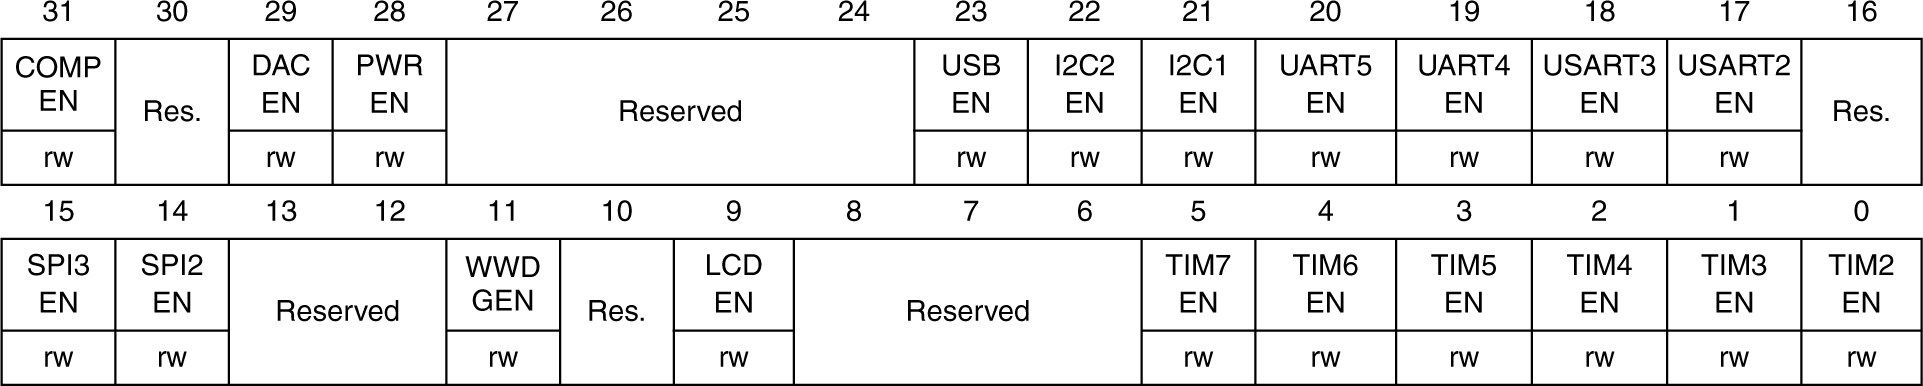
\includegraphics[scale=0.25]{Image/46.jpg} 
\end{center}
\caption{Регистр \textit{RCC\_APB1ENR} (APB1 peripheral clock enable register)}
\end{figure}

\begin{verbatim}
RCC->APB1ENR |= RCC_APB1ENR_PWREN|RCC_APB1ENR_LCDEN;

// RCC->APB1ENR |= 0x10000200;
// 0x10000200 = 1 0000 0000 0000 0000 0010 0000 0000 
\end{verbatim}

	Для работы контроллера ЖКИ необходимо указать источник тактовых сигналов. Источник указывается в регистре \textit{ RCC\_CSR}. По умолчанию запись в этот регистр запрещена. В регистре управления питанием  \textit{PWR\_CR} (PWR power control register) снимается защита от записи в регистр  \textit{RCC\_CSR}. Регистр  \textit{RCC\_CSR} управляет источниками тактирования часов  \textit{RTC }и контроллера ЖКИ.

\begin{figure}[H]
\begin{center}
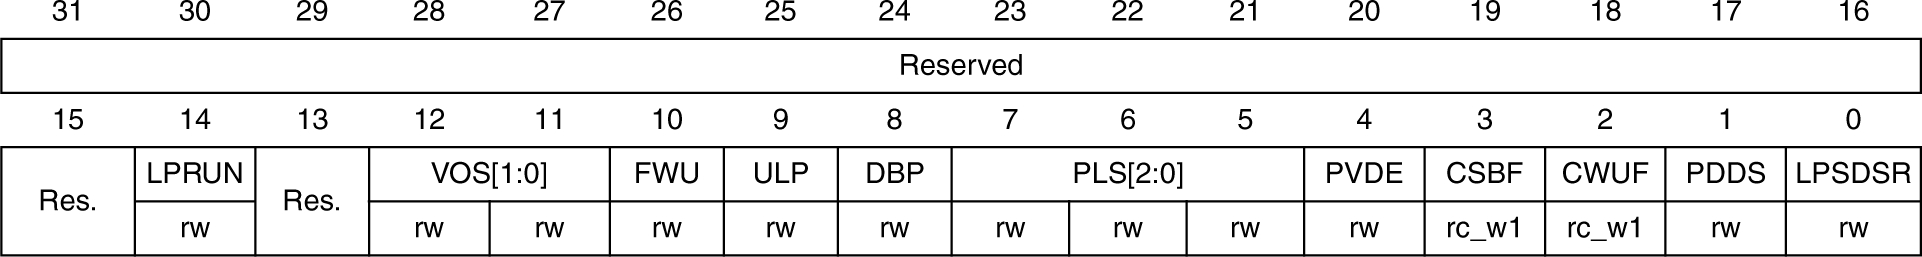
\includegraphics[scale=0.25]{Image/47.jpg} 
\end{center}
\caption{Регистр \textit{PWR\_CR} (PWR power control register)}
\end{figure}

Запись в регистр \textit{ RCC\_CSR} разрешается установкой \verb\1\ в 8 разряд регистра \textit{PWR\_CR}. 

\begin{verbatim}
PWR->CR |= PWR_CR_DBP; 

// PWR->CR |= 0x100;
// 0x100 = 1 0000 0000 
\end{verbatim}


Для смены источника тактирования контроллера ЖКИ (и часов RTC тоже) необходимо сначала выполнить сброс источника тактирования установкой бита \textit{RTCRST} (установкой \verb\1\ в 23 разряд) в регистре \textit{ RCC\_CSR} (Control/status register). 

\begin{figure}[H]
\begin{center}
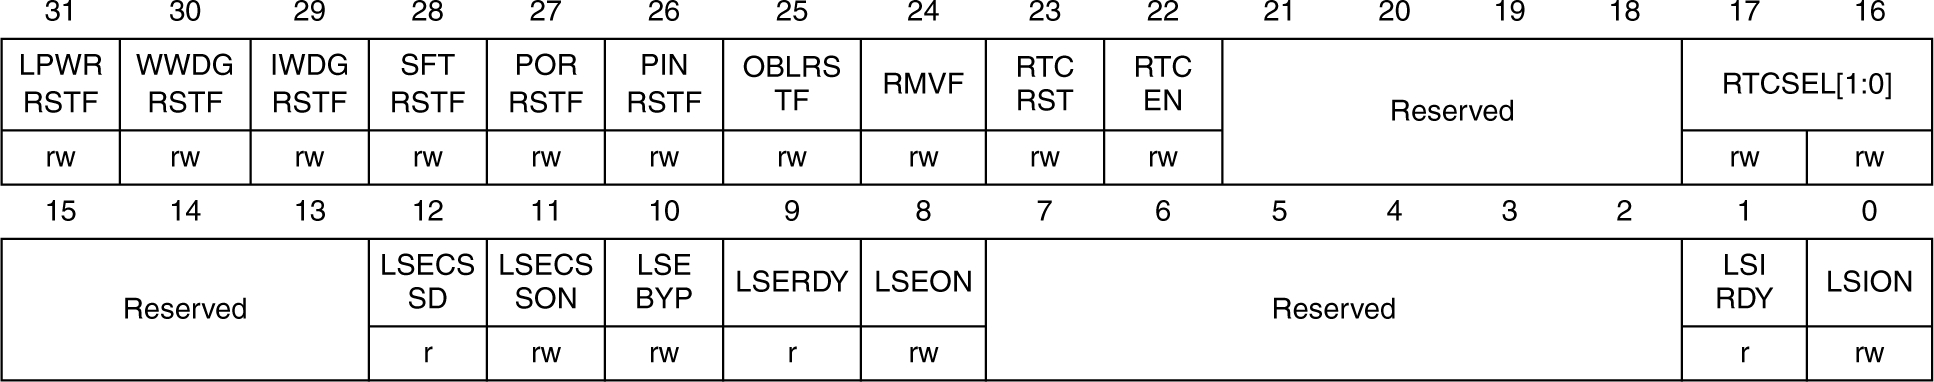
\includegraphics[scale=0.25]{Image/48.jpg} 
\end{center}
\caption{Регистр \textit{ RCC\_CSR}(Control/status register)}
\end{figure}

\begin{verbatim}
RCC->CSR |= RCC_CSR_RTCRST;

// RCC->CSR |= 0x800000;
// 0x800000 = 1000 0000 0000 0000 0000 0000 
\end{verbatim}
Для выбора нового источника тактирования необходимо убрать бит  \textit{RTCRST}:
\begin{verbatim}
RCC->CSR &= ~RCC_CSR_RTCRST;

// RCC->CSR &= ~0x800000;
\end{verbatim}
В качестве источника тактового сигнала выбирается внешний НЧ генератор. Для включения генератора в регистре \textit{ RCC\_CSR} необходимо установить бит \textit{LSEON} (установить \verb\1\ в 8 разряд):
\begin{verbatim}
RCC->CSR |= RCC_CSR_LSEON; 

// RCC->CSR |= 0x100; 
// 0x100 = 1 0000 0000
\end{verbatim}
После включения генератора необходимо некоторое время на его стабилизацию. Готовность генератора проверяется аппаратной установкой бита \textit{LSERDY} в регистре \textit{ RCC\_CSR}:
\begin{verbatim}
while(!(RCC->CSR&RCC_CSR_LSERDY));
\end{verbatim}
Выбор внешнего НЧ генератора в качестве источника тактового сигнала осуществляется установкой в группе \textit{RTCSEL[1:0]} регистра \textit{ RCC\_CSR} значения \verb\01\:
\begin{verbatim}
RCC->CSR |= RCC_CSR_RTCSEL_LSE;

// RCC->CSR |= 0x10000; 
// 0x10000 = 1 0000 0000 0000 0000
\end{verbatim}
В контроллере ЖКИ необходимо установить нужный режим \textit{bias}. Для этого в регистре \textit{LCD\_CR} (LCD control register) необходимо установить значение \verb\10\ в группу \textit{BIAS[1:0]}. Перед установкой бит необходимо очистить биты от <<мусора>>:
\begin{verbatim}
LCD->CR &= ~LCD_CR_BIAS;

// LCD->CR &= ~0x60;
\end{verbatim}
Выбор режима \textit{bias=1/3}:
\begin{verbatim}
LCD->CR |= LCD_CR_BIAS_1;

// LCD->CR |= 0x40;
\end{verbatim}
Устанавливаем режим \textit{duty=1/4}. Для этого также вначале сбрасываем все биты:
\begin{verbatim}
LCD->CR &=~LCD_CR_DUTY; 

// LCD->CR &= ~0x1C;
\end{verbatim}
Устанавливаем значение \verb\011\ в группу \textit{DUTY[1:0]} регистра \textit{LCD\_CR} для режима \textit{duty=1/4}:
\begin{verbatim}
LCD->CR |= LCD_CR_DUTY_0|LCD_CR_DUTY_1;

// LCD->CR |= 0xС;
\end{verbatim}

\begin{figure}[H]
\begin{center}
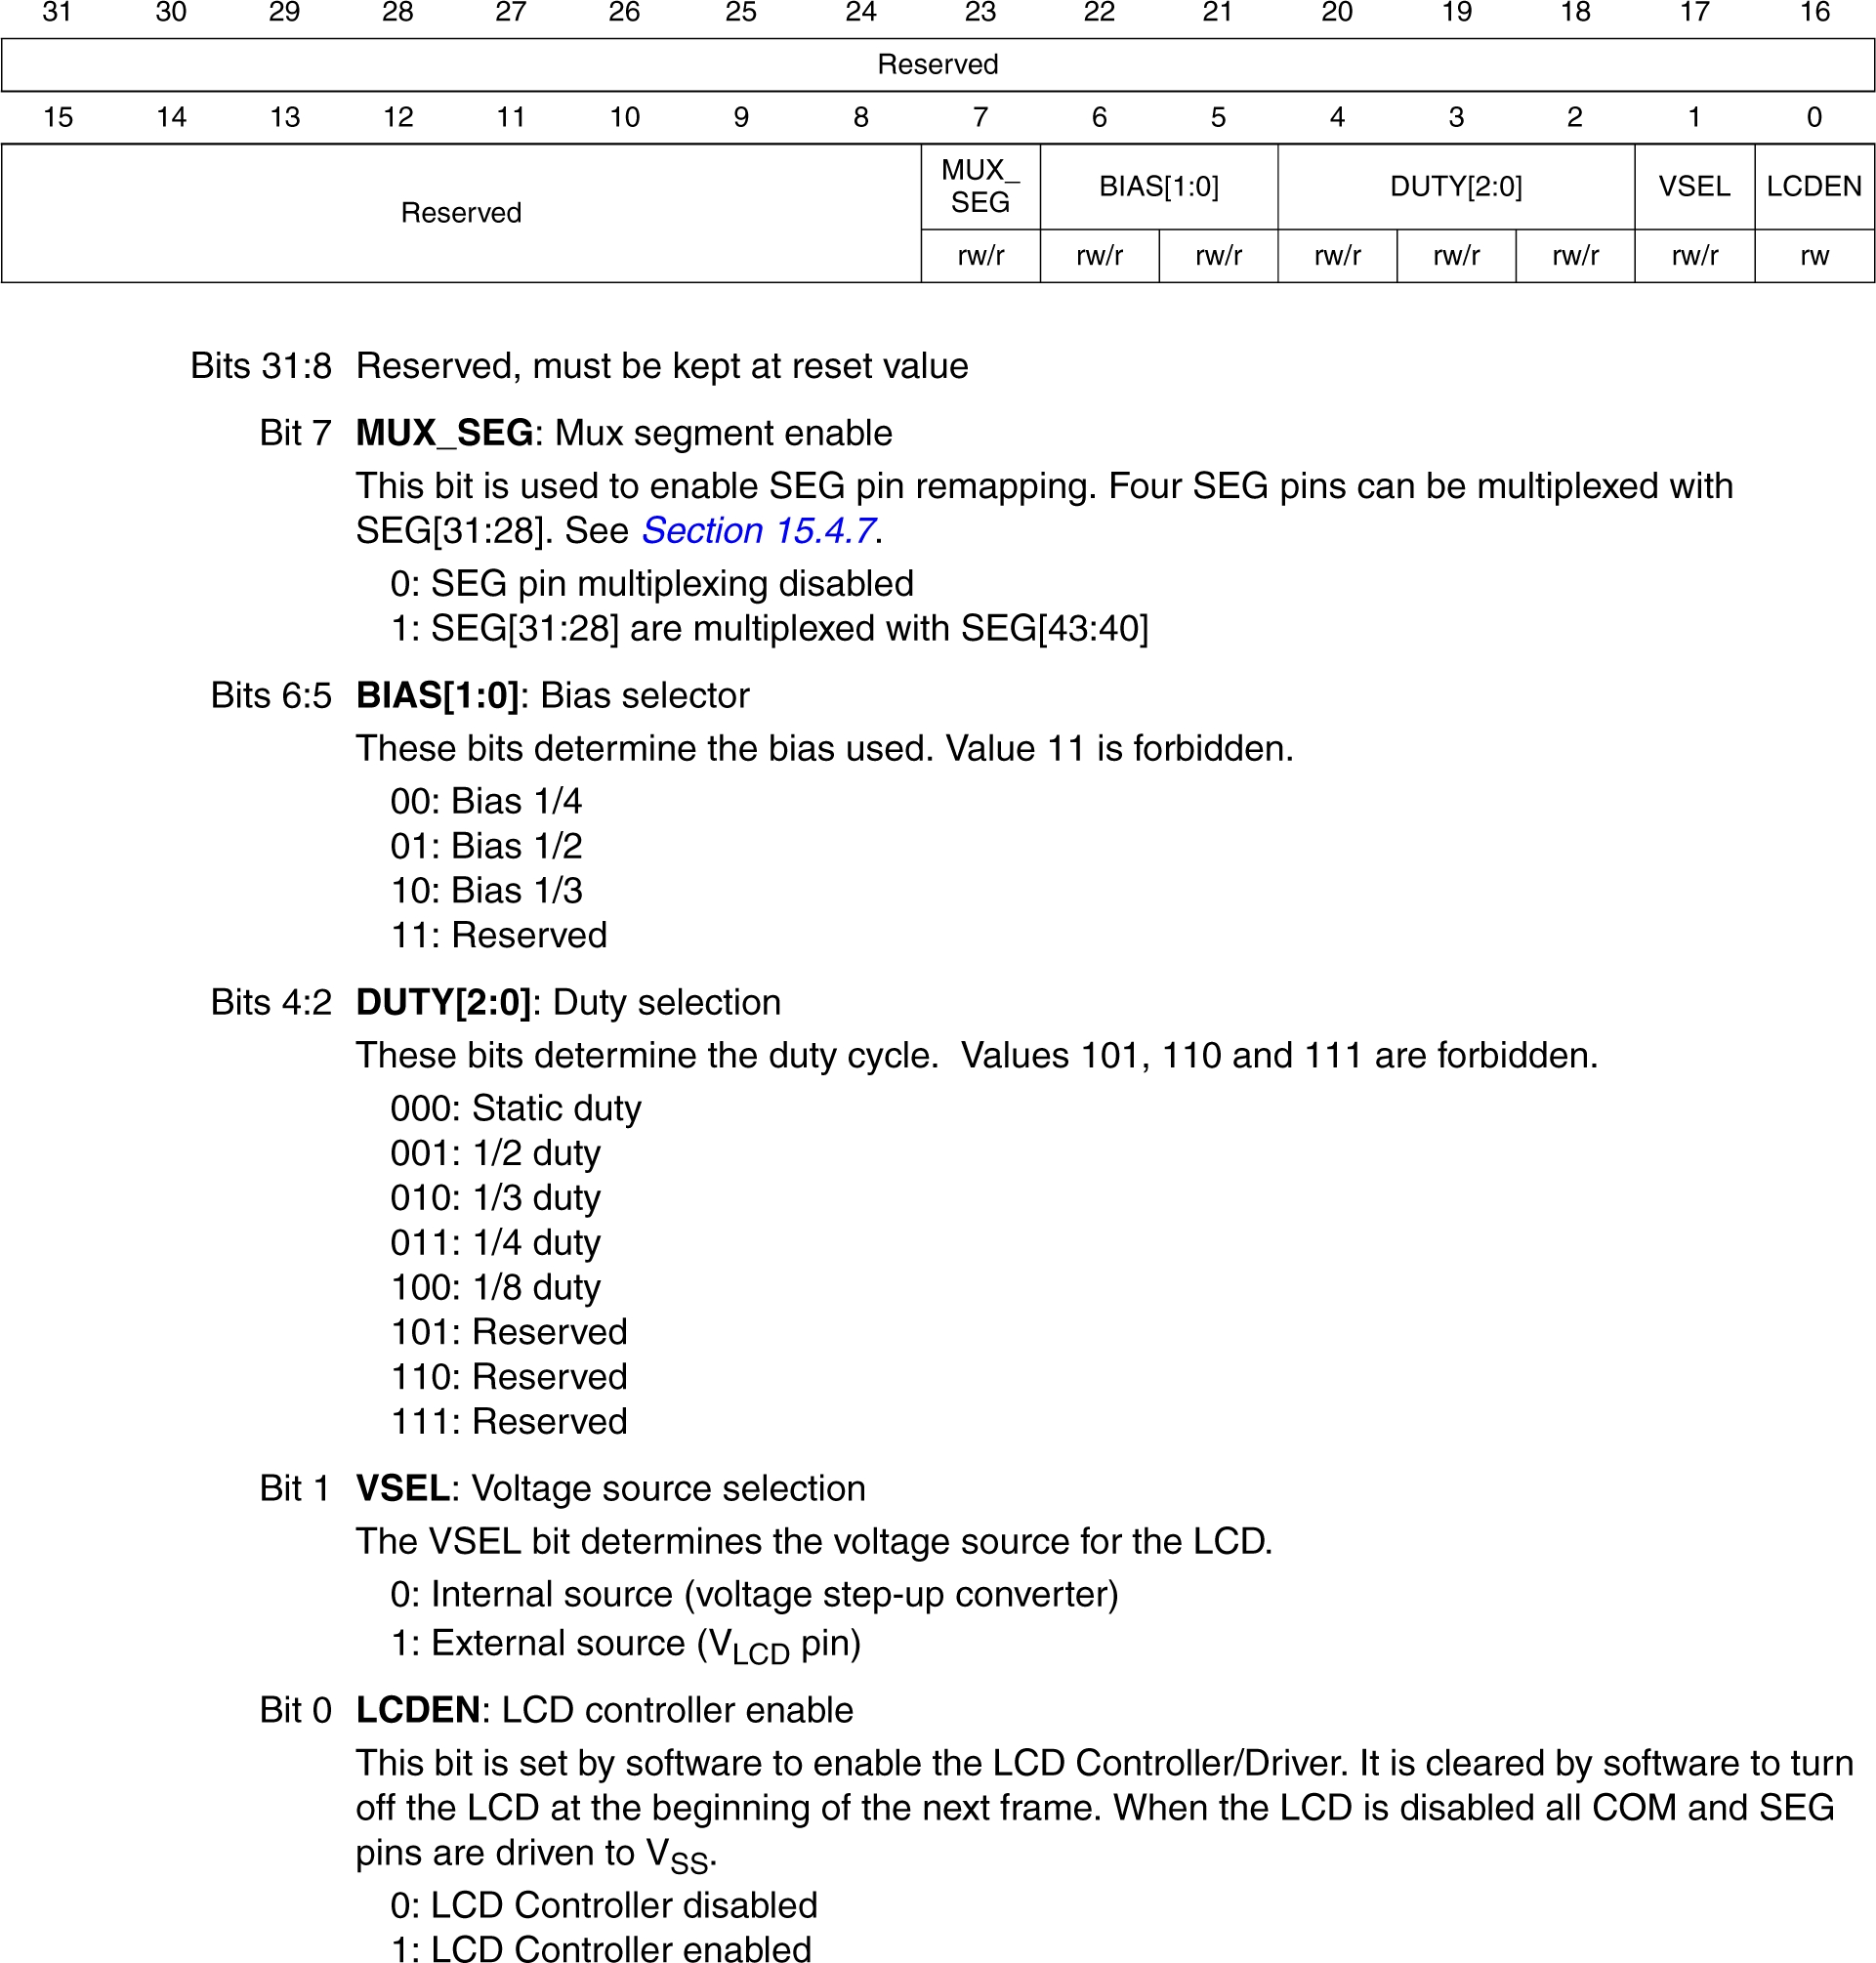
\includegraphics[scale=0.25]{Image/49.jpg} 
\end{center}
\caption{Регистр \textit{LCD\_CR} (LCD control register)}
\end{figure}
Активируем функцию переназначения выводов. Для этого устанавливаем \verb\1\ в 7 разряд регистра \textit{LCD\_CR}:
\begin{verbatim}
LCD->CR |= LCD_CR_MUX_SEG; 

// LCD->CR |= 0x80;
\end{verbatim}
Устанавливаем значения коэффициентов деления частоты тактового сигнала \textit{LCDCLK}. Значения коэффициентов выставляются в регистре \textit{LCD\_FCR} (LCD frame control register). Вначале также очищаем все биты, затем устанавливаем нужные. 
\begin{verbatim}
LCD->FCR &= ~LCD_FCR_PS;
LCD->FCR &= ~LCD_FCR_DIV;

// LCD->FCR &= ~0x3C00000;
// LCD->FCR &= ~0x3C0000;
\end{verbatim}
\begin{figure}[H]
\begin{center}
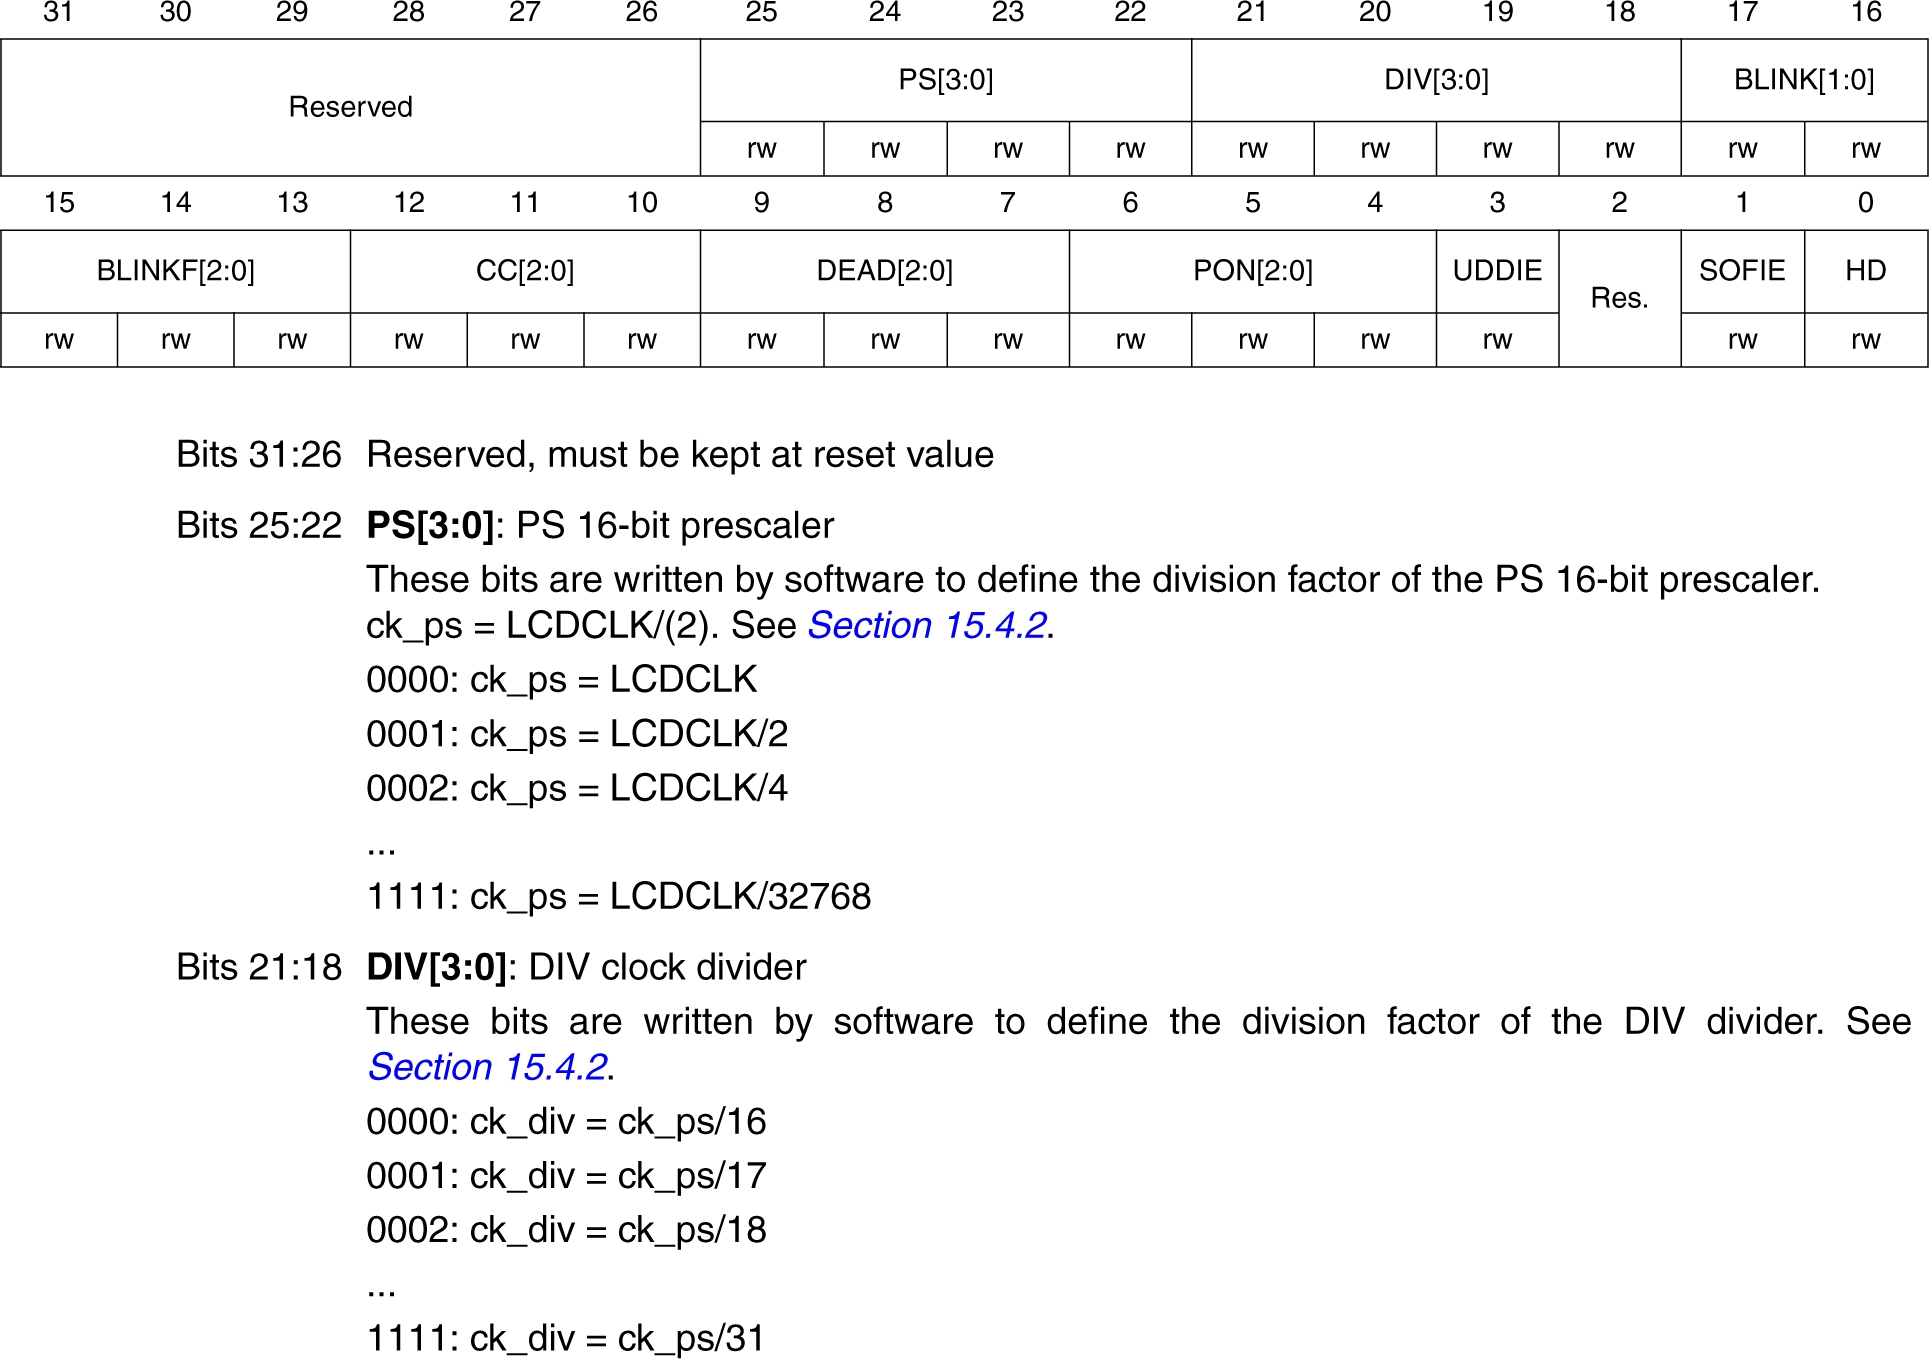
\includegraphics[scale=0.25]{Image/50.jpg} 
\end{center}
\caption{Регистр \textit{LCD\_FCR} (LCD frame control register)}
\end{figure}
Значения коэффициентов деления частоты тактового сигнала устанавливаем равными \textit{ck\_ps = LCDCLK/16, ck\_div = ck\_ps/17}. Для этого устанавливаем \verb\1\ в 24 и в 18 разряды.
\begin{verbatim}
LCD->FCR |= 0x1040000;
// 0x1040000 = 1 0000 0100 0000 0000 0000 0000 
\end{verbatim}
Частоту обновления кадров можно установить больше, например:
\begin{verbatim}
LCD->FCR &= ~0x3C0000;
\end{verbatim}
В это случае, при использовании библиотечных функций вывода изображений на ЖКИ, задержка обновления информации будет менее выражена, однако на ЖКИ будут видны артефакты.

Для установки нужного уровня контраста необходимо установить значение \verb\010\ в группу \textit{СС[1:0]}, так же предварительно очистив биты от старых значений:
\begin{verbatim}
LCD->FCR &= ~LCD_FCR_CC;  
LCD->FCR |= LCD_FCR_CC_1; 

// LCD->FCR &= ~0x1C00;
// LCD->FCR |= 0x800;
// 0x800 = 1000 0000 0000
\end{verbatim}
После установки всех значений необходимо некоторое время на синхронизацию регистра \textit{LCD\_FCR}. Синхронизация регистра проверяется аппаратной установкой бита \textit{FCRSF} в регистре \textit{LCD\_SR} (LCD status register).
\begin{verbatim}
while(!(LCD->SR&LCD_SR_FCRSR)); 
\end{verbatim}
\begin{figure}[H]
\begin{center}
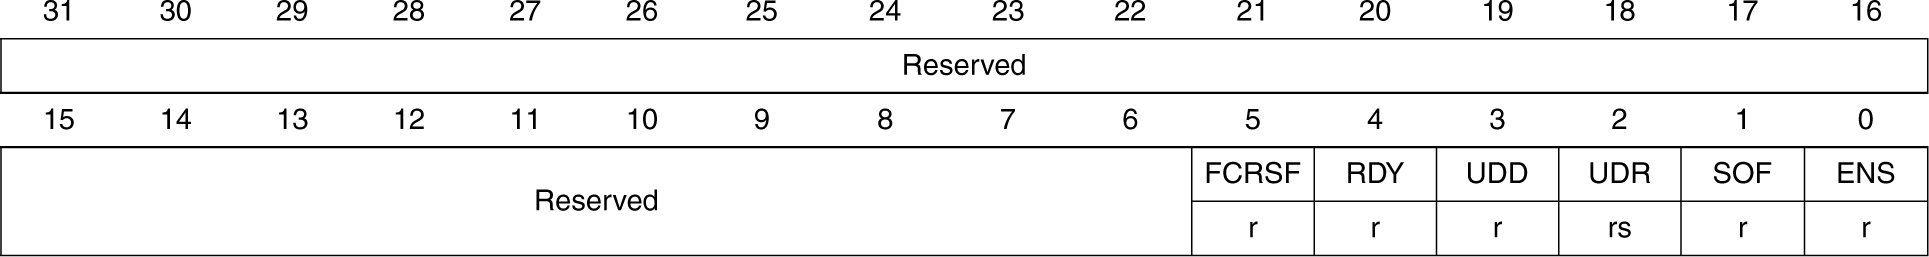
\includegraphics[scale=0.25]{Image/51.jpg} 
\end{center}
\caption{Регистр \textit{LCD\_SR} (LCD status register)}
\end{figure}
В качестве источника напряжения для ЖКИ выбираем внутренний \textit{step-up converter} для формирования \textit{V\_lcd}.  Для этого в первый разряд регистра \textit{LCD\_CR} (LCD control register) устанавливается значение \verb\0\:
\begin{verbatim}
LCD->CR &= ~LCD_CR_VSEL; 

//LCD->CR &= ~0x2;
\end{verbatim}
Разрешение работы ЖКИ контроллера происходит установкой \verb\1\ в 0 разряд регистра \textit{LCD\_CR} (LCD control register):
\begin{verbatim}
LCD->CR |= LCD_CR_LCDEN;

//LCD->CR |= 0x1;
\end{verbatim}
После установки в качестве источника напряжения внутреннего \textit{step-up converter}, необходимо дождаться его готовности. Готовность проверяется аппаратной установкой бита \textit{RDY} в регистре \textit{LCD\_SR} (LCD status register).
\begin{verbatim}
while(!(LCD->SR&LCD_SR_RDY)); 
\end{verbatim}
После разрешения работы контроллера ЖКИ, необходимо дождаться его готовности. Готовность проверяется аппаратной установкой бита \textit{ENS} в регистре \textit{LCD\_SR} (LCD status register).
\begin{verbatim}
while(!(LCD->SR&LCD_SR_ENS));
\end{verbatim}






\section{Формирование изображения на ЖКИ}



\subsection{Вывод информации на ЖКИ с использованием регистров \textit{LCD\_RAM}}
\begin{figure}[H]
\begin{center}
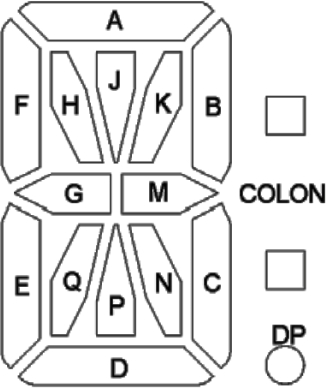
\includegraphics[scale=0.4]{Image/52.jpg} 
\end{center}
\caption{Обозначение сегментов}
\end{figure}
Все сегменты индикатора объединены в группы COM0 -- COM3 по 24 сегмента в каждой (SEG0 -- SEG23). Информация о сегментах хранится в регистрах \textit{LCD\_RAM} памяти контроллера ЖКИ. Разводка печатной платы такова, что номера сегментов не соответствуют номерам разрядов регистров \textit{LCD\_RAM}.

В качестве примера рассмотрим вывод на ЖКИ слова \verb#KAF403#.
\begin{figure}[H]
\begin{center}
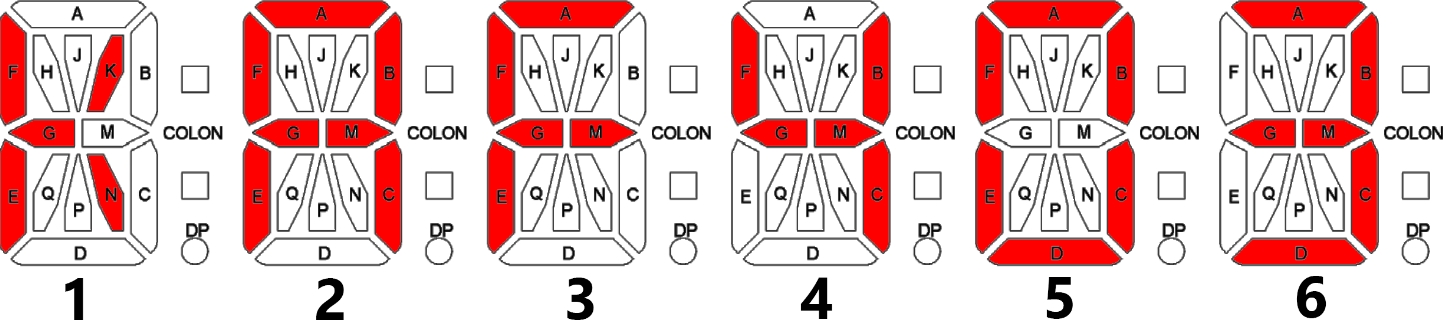
\includegraphics[scale=0.33]{Image/53.jpg} 
\end{center}
\caption{Вывод на ЖКИ}\label{kaf403}
\end{figure}
Для вывода данного слова необходимо (см. рисунок \ref{segment}) зажечь сегменты: 
\begin{itemize}
\item 1G, 1E, 2B, 2M, 2G, 2E, 3M, 3G, 3E, 4M, 4G, 5B, 5E, 6B, 6M, 6G принадлежащие группе COM0 (см. также рисунок \ref{SegmentTable});
\item 1F, 2A, 2F, 2C, 3A, 3F, 4F, 4C, 5A, 5F, 5C, 5D, 6A, 6C, 6D принадлежащие группе COM1;
\item 1K принадлежащие группе COM2;
\item 1N принадлежащие группе COM3;
\end{itemize}
Что бы зажечь выбранные сегменты, необходимо установиться 1 в соответствующих разрядах регистров \textit{LCD\_RAM}, принадлежащих определенной группе COM. Разряд регистра определяется в соответствии с таблицей на рисунке \ref{kaf403}.  
\begin{figure}[H]
\begin{center}
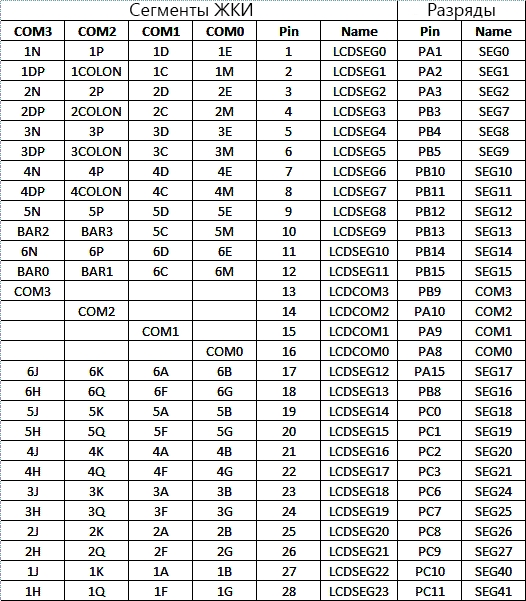
\includegraphics[scale=0.8]{Image/54.jpg} 
\end{center}
\caption{Таблица сегментов}\label{SegmentTable}
\end{figure}
К примеру сегмент 1G подключен к выводу \textit{LSDSEG23} ЖКИ, за данный сегмент отвечает разряд \textit{SEG41}. Сегмент 1G принадлежит группе COM0 и за него отвечает разряд \textit{SEG41}, следовательно информация о нем должна быть записана в регистр \textit{LCD\_RAM[1]} (см. рисунок \ref{COM0}), но поскольку используется функция переназначения (remapping), то информация будет записана в разряд \textit{SEG29} регистра \textit{LCD\_RAM[0]} (см. страницу \pageref{RegMemLCD}). 

Сегмент 1Е подключен к выводу \textit{LSD\_SEG0} ЖКИ, за данный сегмент отвечает разряд \textit{SEG0}. Данный сегмент принадлежит группе COM0 и информация будет записана в регистр \textit{LCD\_RAM[0]}.

Сегмент 2B подключен к выводу \textit{LSD\_SEG20} ЖКИ, за данный сегмент отвечает разряд \textit{SEG26}. Данный сегмент принадлежит группе COM0 и информация будет записана в регистр \textit{LCD\_RAM[0]}.

Сегмент 2M подключен к выводу \textit{LSD\_SEG3} ЖКИ, за данный сегмент отвечает разряд \textit{SEG7}. Данный сегмент принадлежит группе COM0 и информация будет записана в регистр \textit{LCD\_RAM[0]}.

Сегмент 2G подключен к выводу \textit{LSD\_SEG21} ЖКИ, за данный сегмент отвечает разряд \textit{SEG27}. Данный сегмент принадлежит группе COM0 и информация будет записана в регистр \textit{LCD\_RAM[0]}.

Сегмент 2E подключен к выводу \textit{LSD\_SEG2} ЖКИ, за данный сегмент отвечает разряд \textit{SEG2}. Данный сегмент принадлежит группе COM0 и информация будет записана в регистр \textit{LCD\_RAM[0]}. 

Сегмент 1K подключен к выводу \textit{LSD\_SEG22} ЖКИ, за данный сегмент отвечает разряд \textit{SEG40}. C использованием функции переназначения информация должна быть записана в разряд \textit{SEG28}. 

Данный сегмент принадлежит группе COM2 и информация будет записана в регистр \textit{LCD\_RAM[4]}. 
Разряды для других сегментов определяются аналогично.

Далее исходя из полученных разрядов формируется двоичный код, который состоит из 1 в тех разрядах, которые соответствуют определенным ранее \textit{SEGx}. Полученный код записывается также в определенные ранее \textit{LCD\_RAM[x]}. В данной примере регистр \textit{LCD\_RAM[4]} (принадлежащий группе COM2) отвечает только за один сегмент 1K, 1 будет стоять в 28 разряде. В данный регистр будет записан следующий код:
\begin{verbatim}
LCD->RAM[4] = 0x10000000;
// 1 0000 0000 0000 0000 0000 0000 0000_2 = 1000 0000_16
\end{verbatim}
До записи значений в регистры памяти необходимо проверить завершена ли предыдущая передача данных на ЖКИ. Для этого проверяется бит \textit{UDR} (Update display request) регистра \textit{LCD\_SR} (LCD status register). Контроллер ЖКИ имеет два выходных буфера, информация заносится в первый буфер, а выводится на ЖКИ из второго буфера. Бит \textit{UDR} устанавливается во время передачи из первого буфера во второй, защищая от записи регистры \textit{LCD\_RAM}.
\begin{verbatim}
while(LCD->SR & LCD_SR_UDR);
\end{verbatim}
После записи информации в регистры \textit{LCD\_RAM} необходимо установить бит \textit{UDR} в регистре \textit{LCD\_SR} (LCD status register) (установить \verb\1\ во 2 разряд):
\begin{verbatim}
LCD->SR |= LCD_SR_UDR;

// LCD->SR |= 0x4;
// 0x4 = 100
\end{verbatim}

\subsection{Вывод информации на ЖКИ с использованием библиотеки}
В составе \textit{Standard Peripheral Library} (SPL) есть библиотека для работы с LCD дисплеями, состоящая из двух файлов \verb\stm32l1xx_lcd.c\ и \verb\stm32l1xx_lcd.h\. Инициализация контроллера происходит аналогично инициализации портов микроконтроллера в первой лабораторной работе, при помощи структуры. 
\begin{verbatim}
LCD_InitTypeDef LCD_InitStruct; 
LCD_InitStruct.LCD_Prescaler = LCD_Prescaler_1;
LCD_InitStruct.LCD_Divider = LCD_Divider_31;
LCD_InitStruct.LCD_Duty = LCD_Duty_1_4;
LCD_InitStruct.LCD_Bias = LCD_Bias_1_3;
LCD_InitStruct.LCD_VoltageSource = LCD_VoltageSource_Internal;
  
  /* Initialize the LCD */
LCD_Init(&LCD_InitStruct);
LCD_MuxSegmentCmd(ENABLE);  

  /* To set contrast to mean value */
LCD_ContrastConfig(LCD_Contrast_Level_4);

  /* Wait Until the LCD FCR register is synchronized */
LCD_WaitForSynchro();  

  /* Enable LCD peripheral */
LCD_Cmd(ENABLE);  

 /* Wait Until the LCD is enabled */
while(LCD_GetFlagStatus(LCD_FLAG_ENS) == RESET);

  /*!< Wait Until the LCD Booster is ready */ 
while(LCD_GetFlagStatus(LCD_FLAG_RDY) == RESET);

 // LCD_BlinkConfig(LCD_BlinkMode_Off,LCD_BlinkFrequency_Div32);      
LCD_GLASS_Clear();
\end{verbatim}

Стоит отметить, что перед вызовом функции
\begin{verbatim}
void LCD_Init(LCD_InitTypeDef* LCD_InitStruct)
\end{verbatim}
на контроллер ЖКИ необходимо подать тактовый сигнал.

В комплексе с отладочной платой STM32L-Discovery идет демонстрационная прошивка \textit{STM32L\_Discovery\_Firmware\_Pack}, которая также доступна вместе с исходными кодами и библиотеками на официальном сайте STMicroelectronics. В прошивку входят файлы \verb\stm32l_discovery_lcd.c\, \verb\stm32l_discovery_lcd.h\, \verb\discover_board.h\, в которых предоставлен набор удобных функций для работы с ЖКИ, установленным на отладочной плате STM32L-Discovery:

\begin{verbatim}
void LCD_bar(void);
void LCD_GLASS_Init(void);

//Вывод символа в определенном разряде
void LCD_GLASS_WriteChar(uint8_t* ch, bool point, bool column,uint8_t position);

//Вывод строки символов
void LCD_GLASS_DisplayString(uint8_t* ptr);
void LCD_GLASS_DisplayStrDeci(uint16_t* ptr);
void LCD_GLASS_ClearChar(uint8_t position);

//Очистка ЖКИ
void LCD_GLASS_Clear(void);

//Бегущая строка
void LCD_GLASS_ScrollSentence(uint8_t* ptr, uint16_t nScroll, 
                              uint16_t ScrollSpeed);
void LCD_GLASS_WriteTime(char a, uint8_t posi, bool column);
\end{verbatim}